\section{Results}
\label{sec:kstmm:res}

The results for the angular analysis of \BdToKstmm for .38\invfb and 1.0\invfb of data collected at \lhcb are presented below.
A measurement of the differential branching fraction of \BdToKstmm was obtained by fitting
 the invariant mass distribution of selected candidates in each \qsq bin and normalising to \BdToJpsiKstar. 

\subsection{Angular analysis of 0.38\invfb of data}

The invariant mass distribution of the selected \BdToKstmm candidates in the data is shown in Fig.~\ref{fig:res1massfit}.
\begin{figure}[tbp]
\centering
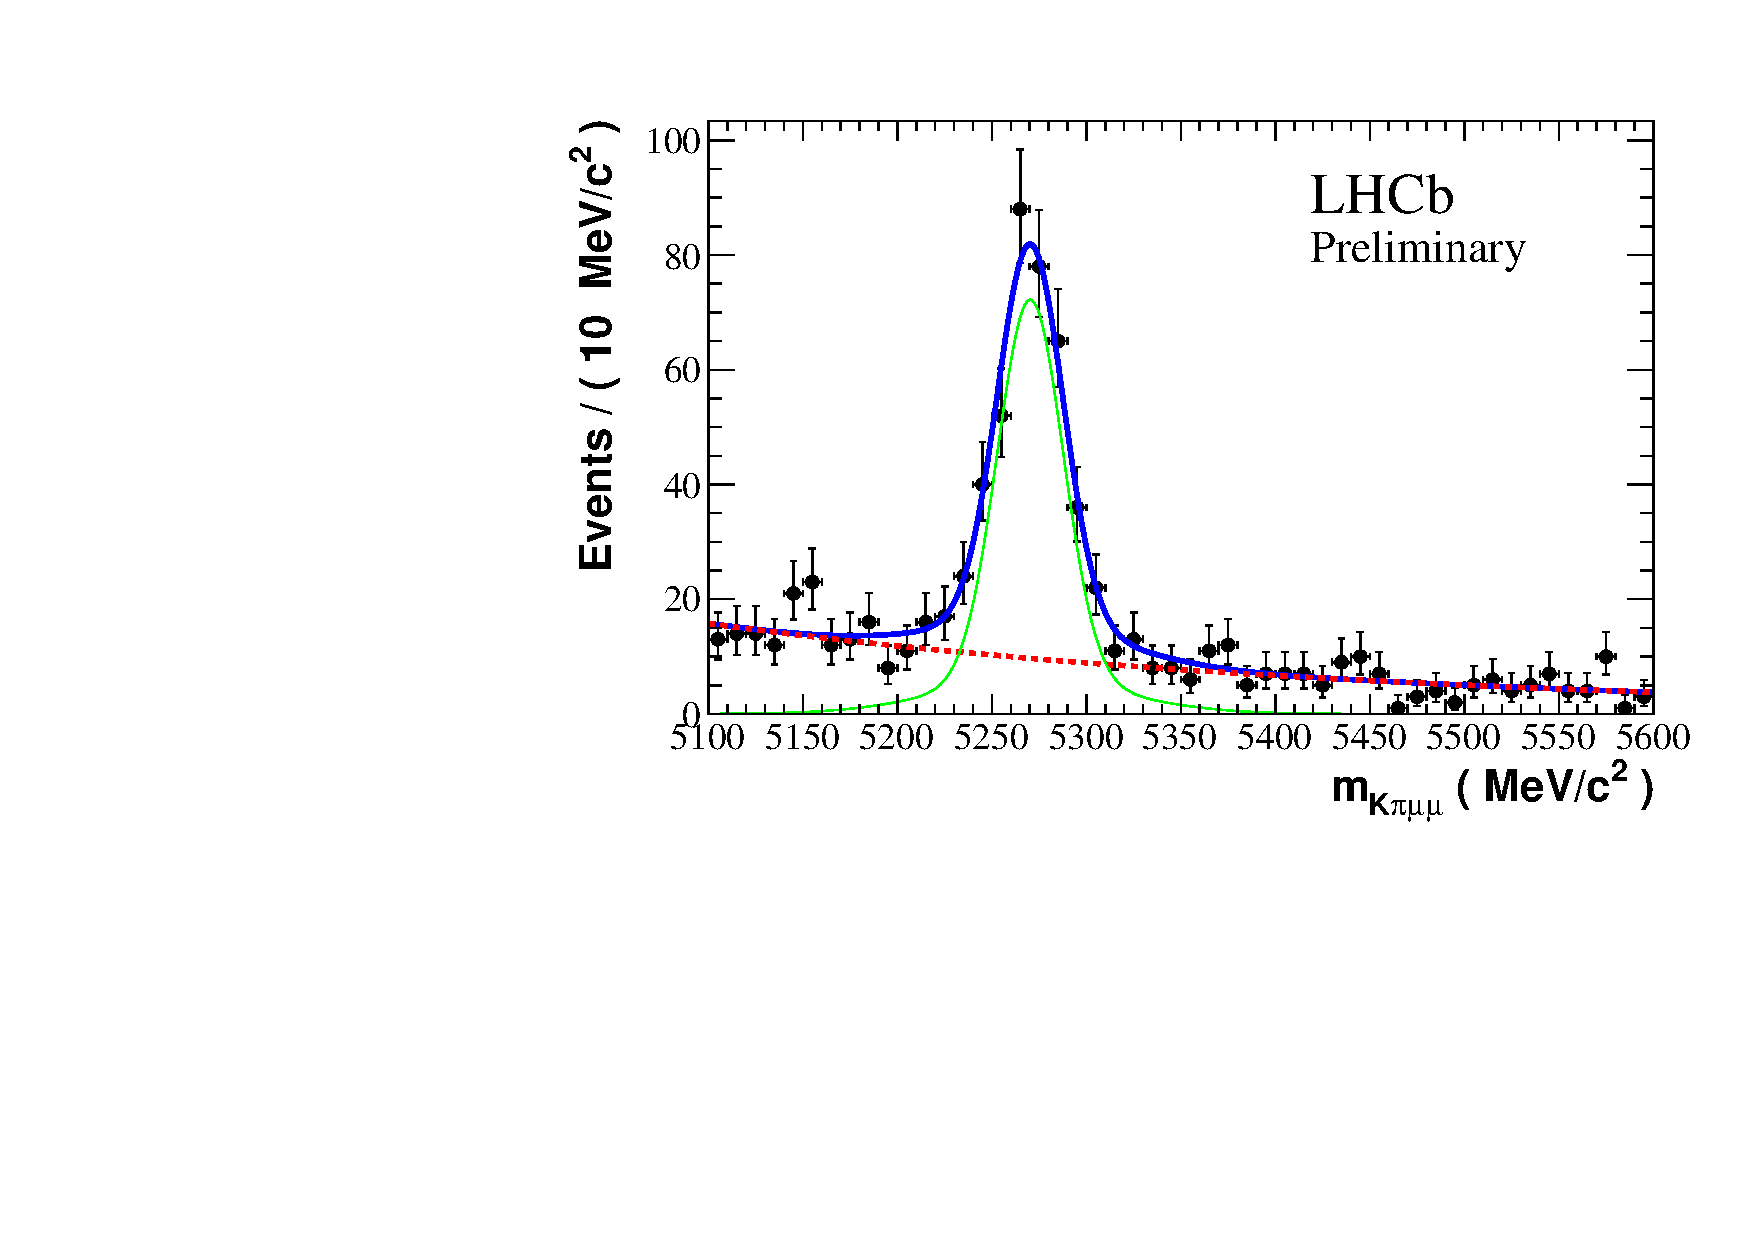
\includegraphics[scale=0.33]{chapter5/figs/results1/mass_fit_full.pdf}
\caption[The fit to the \mkpimm invariant mass distribution of selected \BdToKstmm candidates from 0.37\invfb.]
{The fit to the \mkpimm invariant mass distribution of selected \BdToKstmm candidates from 0.37\invfb.
 The fit to the mass distribution gives an estimate of $337\pm21$ signal events. ~\label{fig:res1massfit}}
\end{figure}
The fit gives an estimate of $337\pm21$ signal events with a background of $97\pm6$ events.
The measured values of \AFB, \FL and the differential branching fraction of \BdToKstmm are shown in Fig.~\ref{fig:kstmm:res1}.
%along with a theoretical prediction from Ref.~\cite{Bobeth:2011gi}. 
\begin{figure}[tbp]
\centering
\subfigure[]{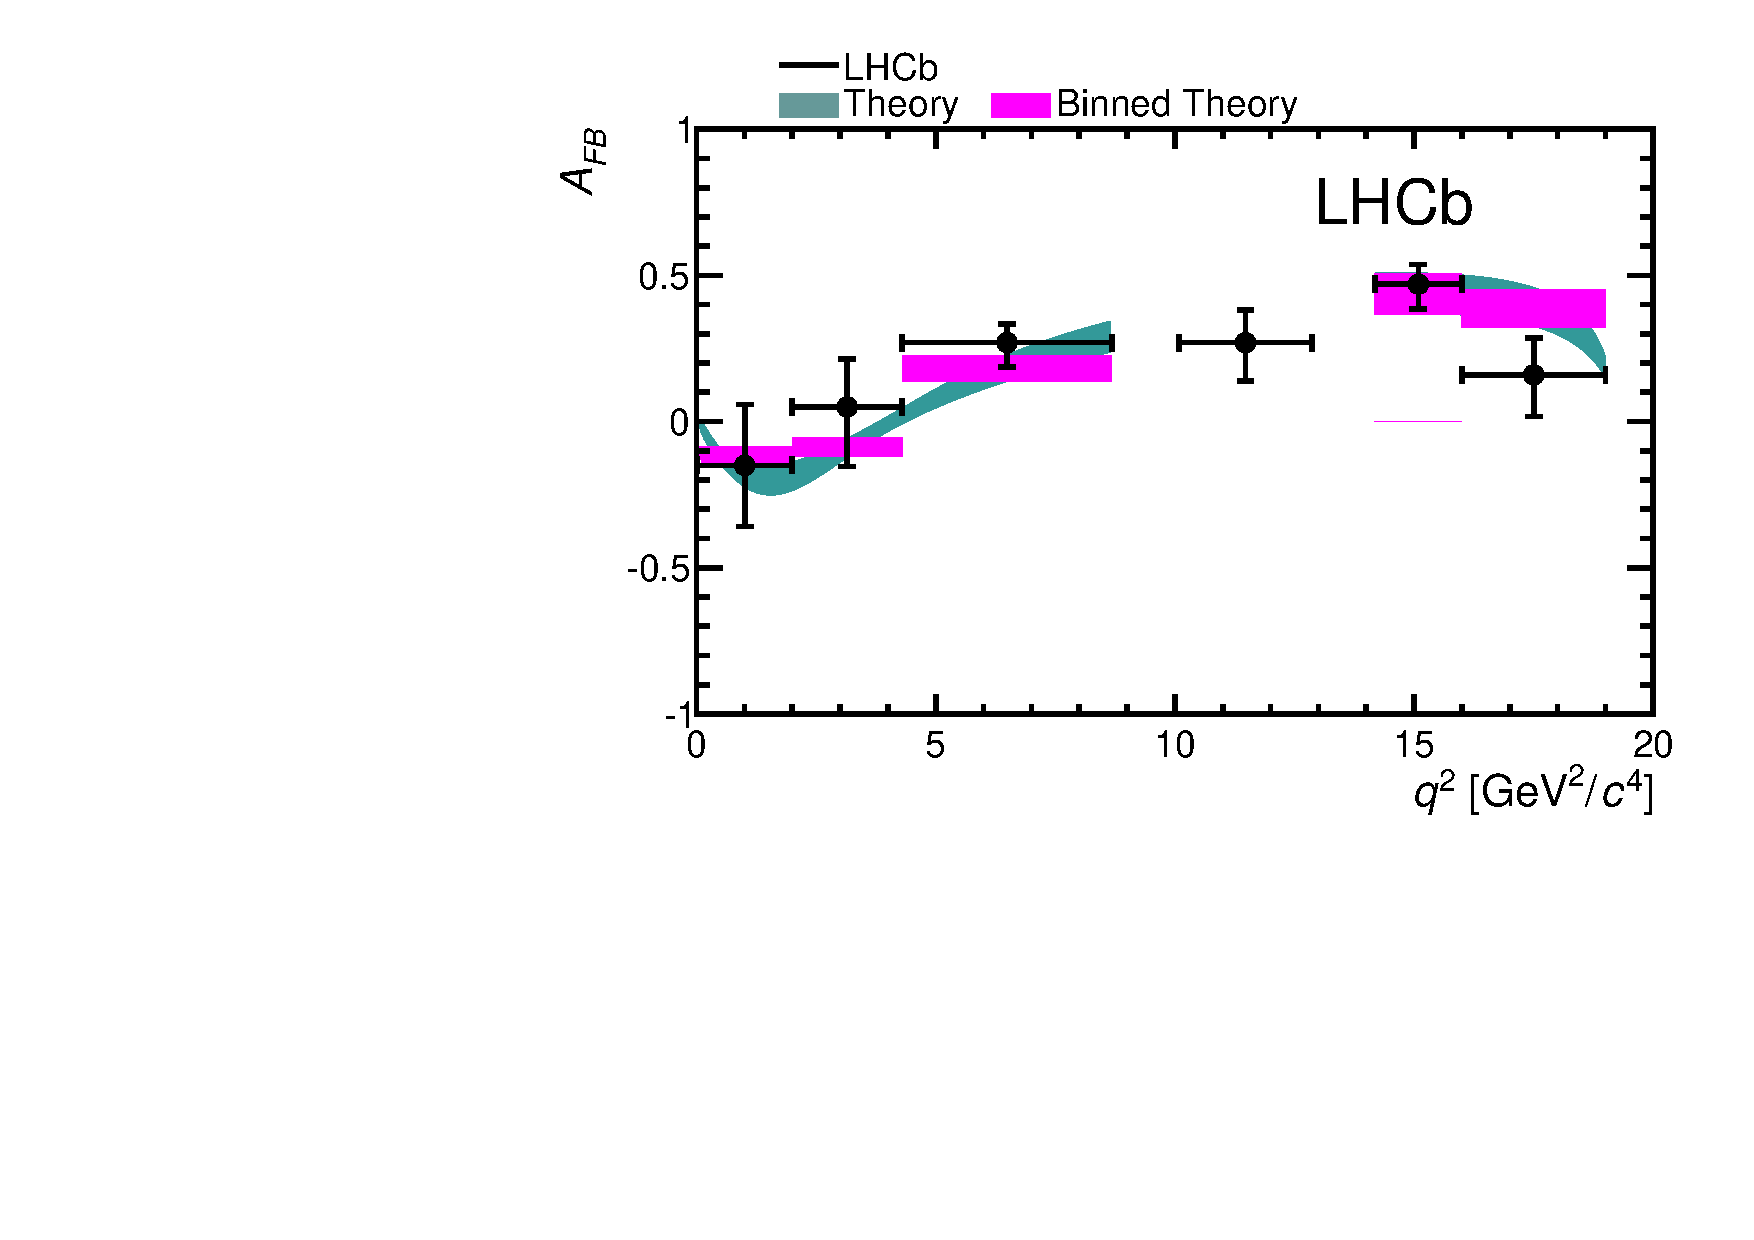
\includegraphics[scale=0.33]{chapter5/figs/results1/plot_AFB1.pdf}}
\subfigure[]{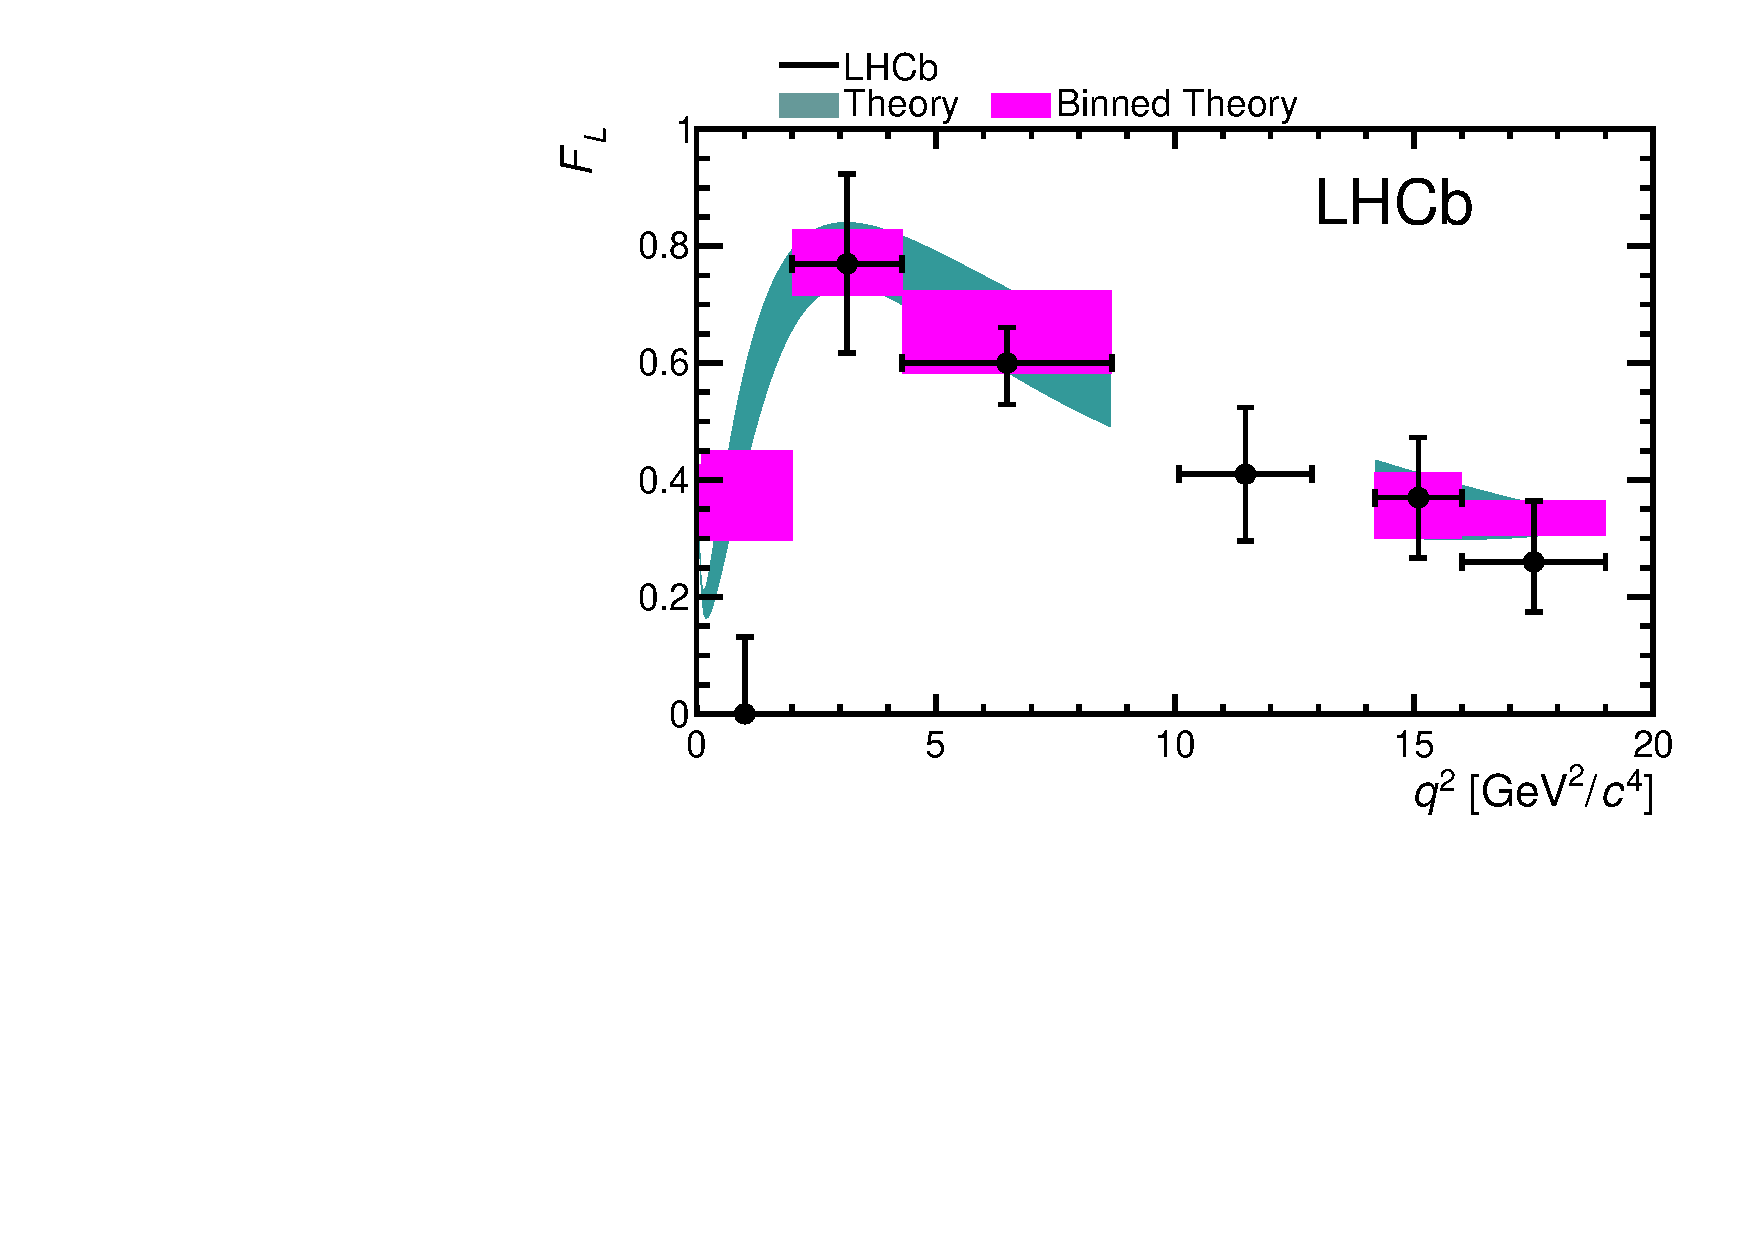
\includegraphics[scale=0.33]{chapter5/figs/results1/plot_FL1.pdf}}
\subfigure[]{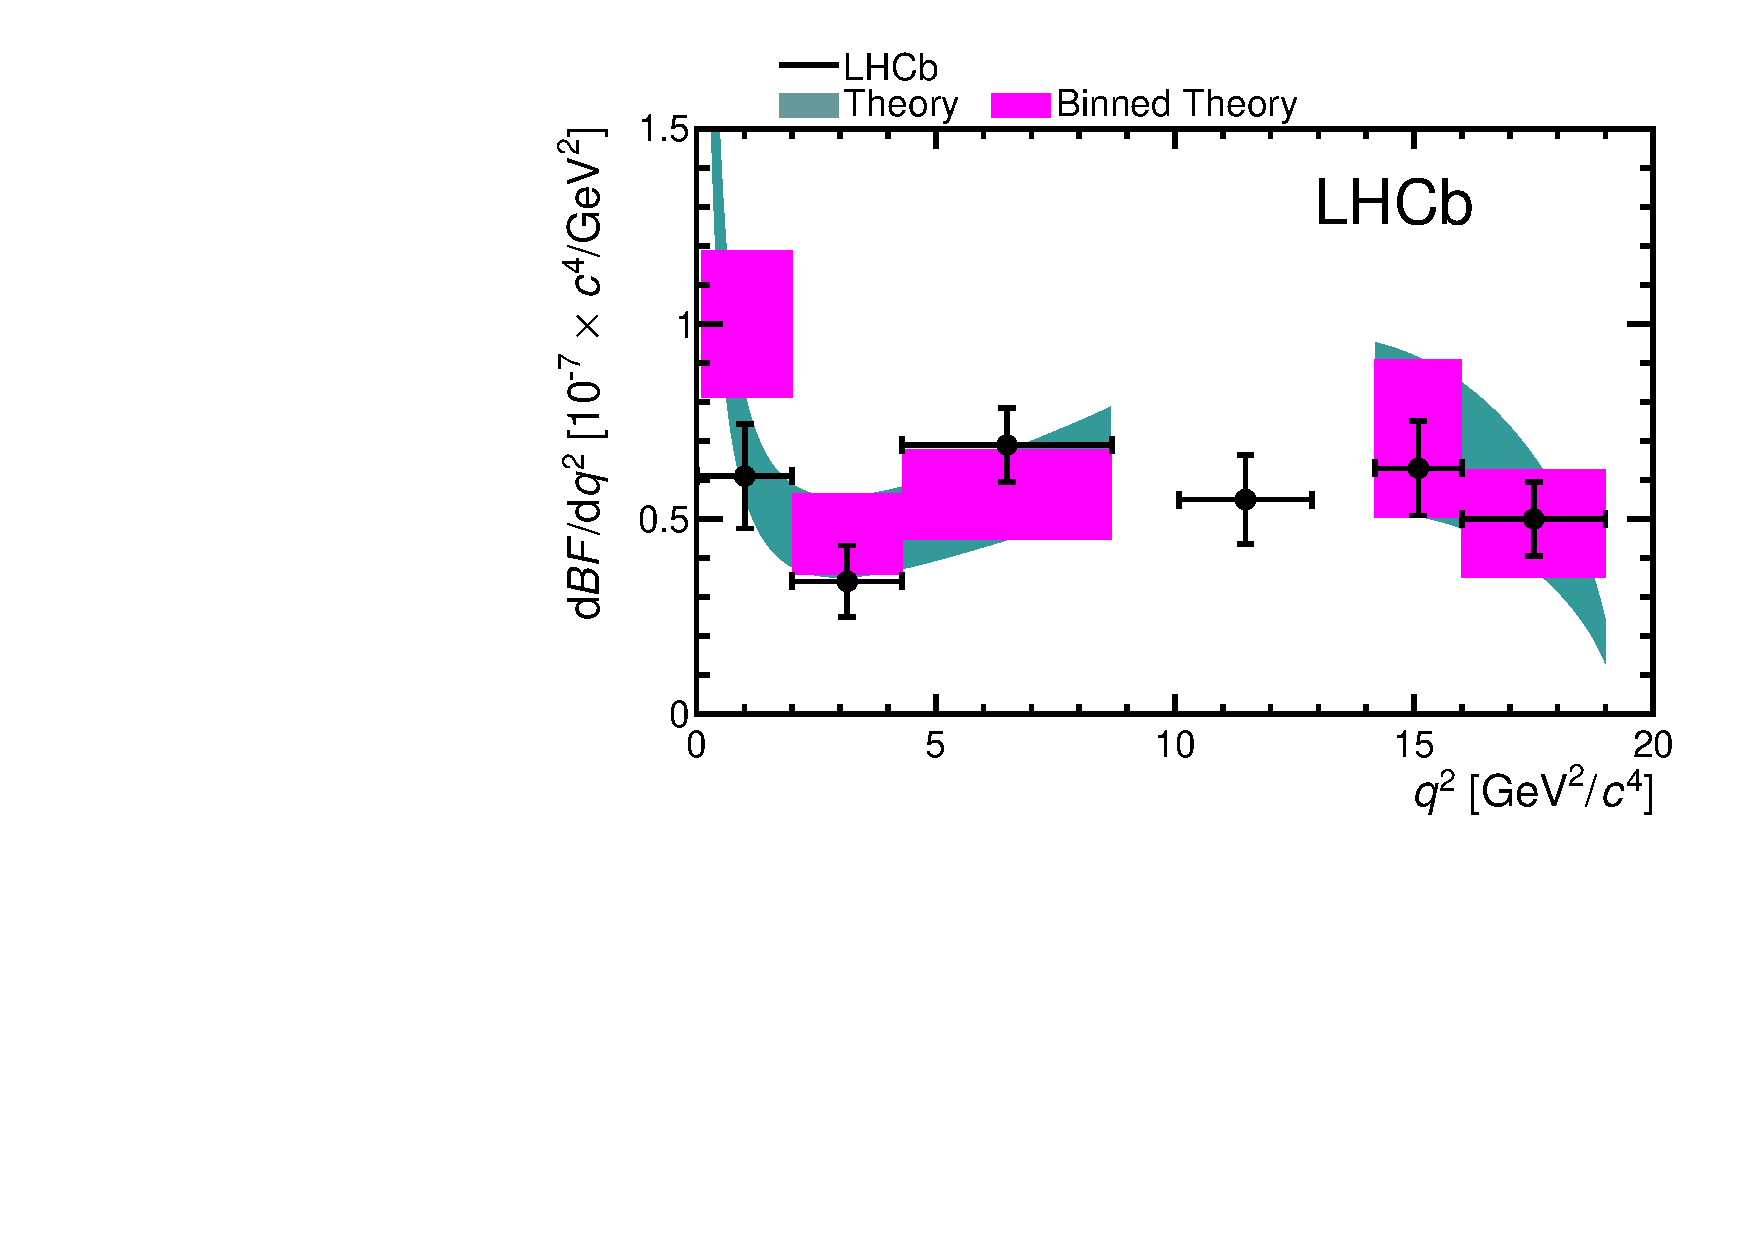
\includegraphics[scale=0.33]{chapter5/figs/results1/plot_Width1.pdf}}
\caption[  The final results from the angular analysis of \BdToKstmm at \lhcb using 0.38\invpb of data collected in 2011 at 7 \tev. ]
{The final results from the angular analysis of \BdToKstmm at \lhcb using 0.38\invpb of data collected in 2011 at 7 \tev. 
Values for \AFB, \FL and the differential branching fraction are extracted in the six different bins of \qsq.
The Standard Model prediction is from~\cite{Bobeth:2011gi}
~\label{fig:kstmm:res1}}
\end{figure}
The central values for the angular observables along with the statistical and systematic errors are given in Table~\ref{table:kstmm:res1}.
\begin{table}[tbp]
\centering
\caption[ The central values and statistical plus systematic uncertainties
 for $A_{FB}$, $F_{L}$ and  $d{\BF}/dq^{2}$ for the 0.38\invfb angular analysis.   ]
{The central values and statistical plus systematic uncertainties
 for $A_{FB}$, $F_{L}$ and  $d{\BF}/dq^{2}$ for the 0.38\invfb angular analysis. 
The first, asymmetric, set of errors is given by the Bayesian error estimate, 
with a prior that the points sit within the physical region. 
The second error is the systematic error on $A_{FB}$, $F_{L}$ and the branching fraction.
\label{table:kstmm:res1}
}
\vspace{5mm}
\begin{tabular}{|c|c|c|c|}
\hline
$\qsq (\gevgevcccc) $ & \AFB & \FL & $d\BF/d\qsq$ ($\times10^{-7} \gev^{-2} c^{4}$)  \\  \hline
$0.10 < q^{2} < 2.00$ & $-0.15^{+0.20}_{-0.20}\pm 0.06$ & $0.00^{+0.13}_{-0.00}\pm 0.02$ & $0.61 \pm 0.12\pm 0.06$ \\
$2.00 < q^{2} < 4.30$ & $+0.05^{+0.16}_{-0.20}\pm 0.04$ & $0.77^{+0.15}_{-0.15} \pm 0.03$ & $0.34 \pm 0.09\pm 0.02$ \\ 
$4.30 < q^{2} < 8.68$ & $+0.27^{+0.06}_{-0.08}\pm 0.02$ & $0.60^{+0.06}_{-0.07} \pm 0.01$ & $0.69 \pm 0.08\pm 0.05$ \\ 
$10.09 < q^{2} < 12.86$ & $+0.27^{+0.11}_{-0.13}\pm 0.02 $ & $0.41^{+0.11}_{-0.11} \pm 0.03$ & $0.55 \pm 0.09\pm 0.07$ \\ 
$14.18 < q^{2} < 16.00$ &  $+0.47^{+0.06}_{-0.08}\pm 0.03$ & $0.37^{+0.09}_{-0.09}\pm 0.05$ & $0.63 \pm 0.11\pm 0.05$ \\ 
$16.00 < q^{2} < 19.00$ & $+0.16^{+0.11}_{-0.13}\pm 0.06$ & $0.26^{+0.10}_{-0.08}\pm 0.03$ & $0.50 \pm 0.08\pm 0.05$ \\
$1.00 < q^{2} < 6.00$ & $-0.06^{+0.13}_{-0.14}\pm 0.04$ & $0.55^{+0.10}_{-0.10}\pm 0.03$ & $0.42 \pm 0.06\pm 0.03$ \\
\hline
\end{tabular}
\end{table}
All of the values for the angular observables lie within the physical limits of \AFB and \FL (Section~\ref{sec:kstmm:obs}) except for the values for the
 $14.18<\qsq<16\gev^2$ bin.
The statistical errors for the physically valid \AFB and \FL values are given by the Bayesian error estimate with a prior that the points sit within the physical region. 
To extract a physical value for the  $14.18<\qsq<16\gev^2$ bin, the lowest value of the likelihood was taken and the errors obtained by integrating 
the likelihood to reach one $\sigma$ coverage.
These were the most precise measurements of the angular observables at the time of publication.


\subsection{Analysis of 1.0\invfb of data}

%The results of the angular analysis of \BdToKstmm at \lhcb using 1.0\invfb of data collected in 2011 are presented below.
The invariant mass distribution of selected \BdToKstmm candidates is shown in Fig.~\ref{fig:res2massfit}  
and there are an estimated $900\pm34$ signal candidates in 1.0\invfb of data. 
\begin{figure}[tbp]
\centering
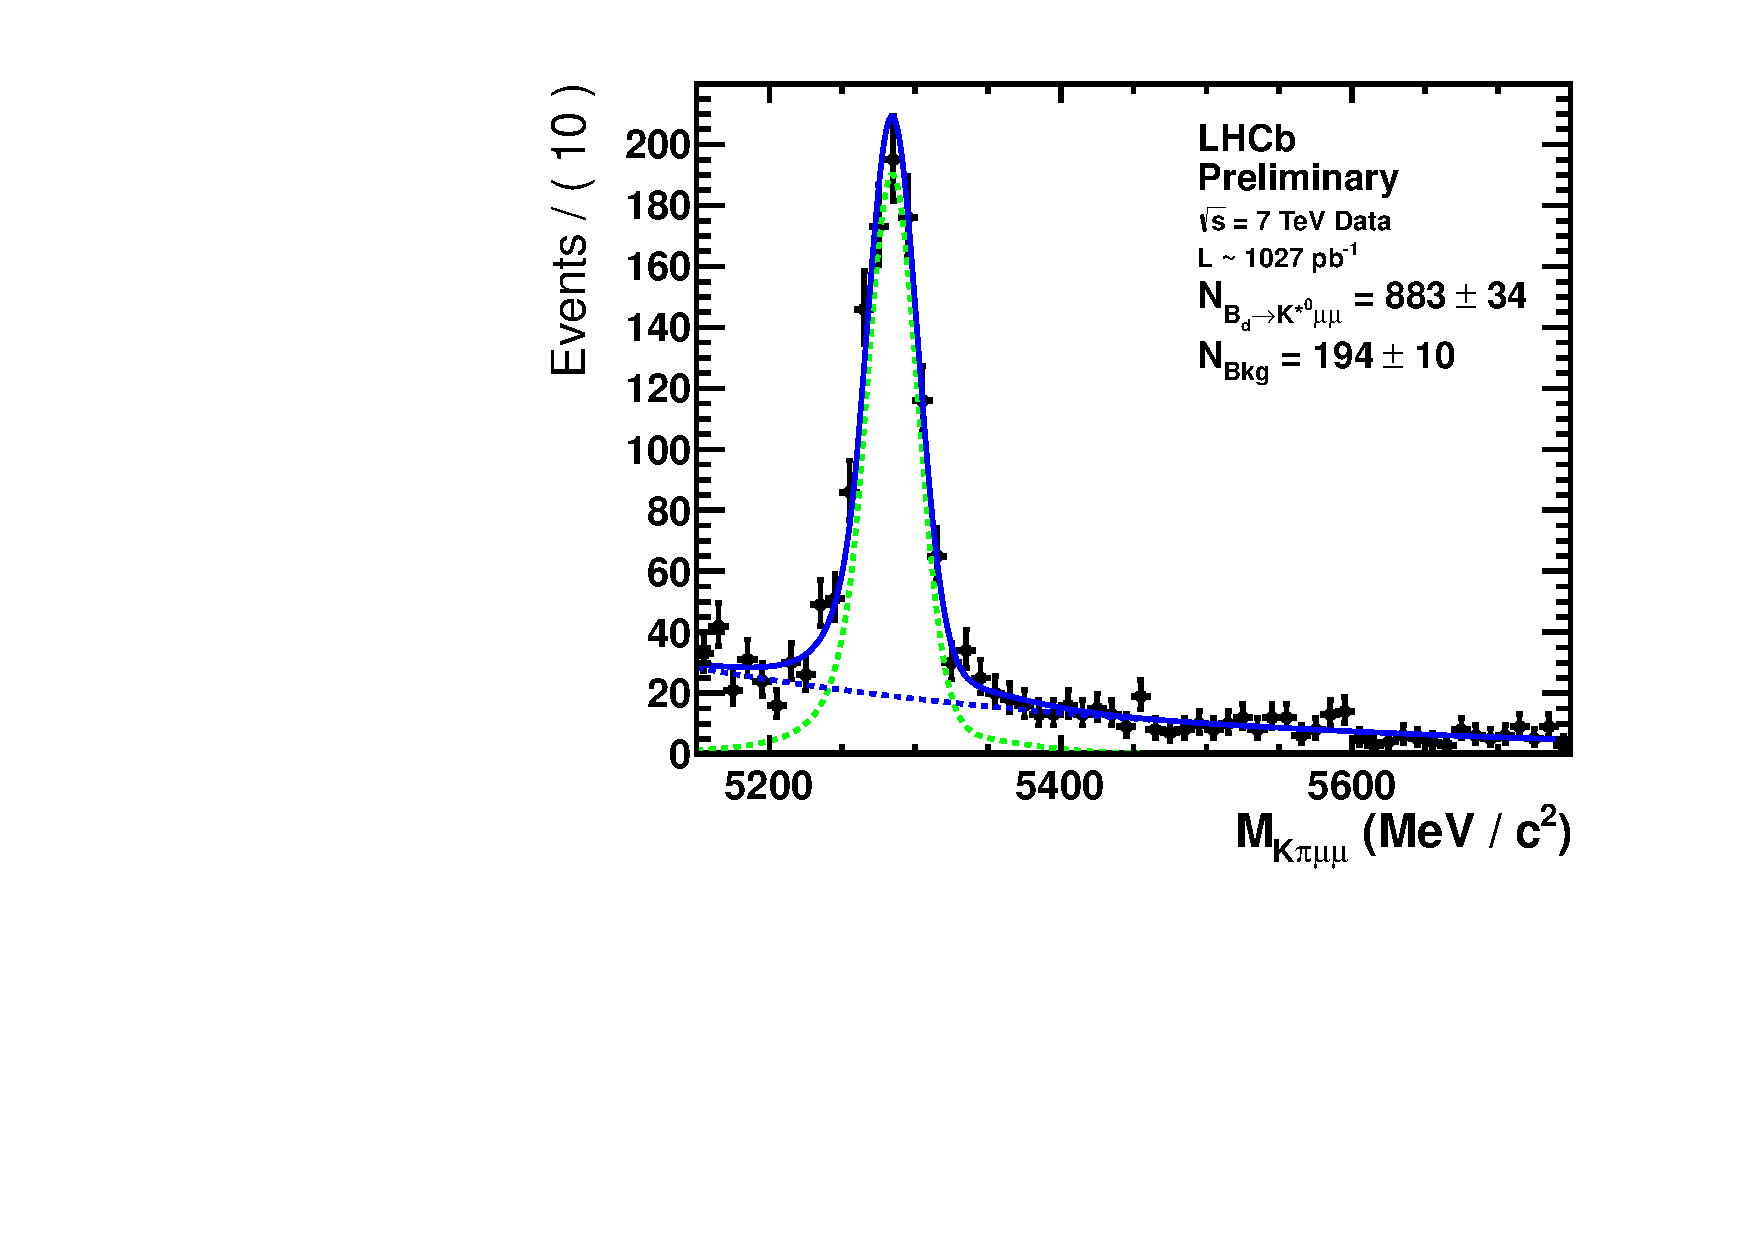
\includegraphics[scale=0.33]{chapter5/figs/results2/KstarMuMuFit_q2low_0_1_q2high_19.pdf}
\caption[ The fit to invariant mass distribution of selected \BdToKstmm candidates from 1.0\invfb of data.  ]
{The fit to invariant mass distribution of selected \BdToKstmm candidates from 1.0\invfb of data.
The fit gives and estimate of $900\pm34$ candidates.~\label{fig:res2massfit}}
\end{figure}
The results for seven angular observables are presented in Table~\ref{table:kstmm:res2}.
The values for the differential branching fraction are presented in Table~\ref{table:kstmm:dbr2}.
\begin{table}[tbp]
\centering
\caption[Fraction of longitudinal polarisation of the \Kstarz, \FL, 
dimuon system forward backward asymmetry, \AFB, and the angular observables 
\OS3, \OS9 and \OA9 from the \BdToKstmm decay in six bins of \qsq.   ]
{Fraction of longitudinal polarisation of the \Kstarz, \FL, 
dimuon system forward backward asymmetry, \AFB, and the angular observables 
\OS3, \OS9 and \OA9 from the \BdToKstmm decay in six bins of \qsq. 
The lower table includes the transverse observables \ATRe and \AT2 
that are thought to have reduced form factor uncertainties. Results are also presented
 in the $1 < \qsq < 6\gevgevcccc$ range where theoretical uncertainties are 
best controlled.  \label{table:kstmm:res2}}
\begin{tabular}{|c|c|c|c|c|} 
\hline
\qsq $(\gevgevcccc)$ & \FL & \AFB & \OS3 & \OS9 \\
\hline
$0.10 - 2.00$ & $0.36\,^{+0.11}_{-0.10}\,^{+0.05}_{-0.03}$ & $-0.02\,^{+0.13}_{-0.12}\,^{+0.03}_{-0.00}$ & $-0.05\,^{+0.09}_{-0.10}\,^{+0.01}_{-0.01}$ & $\phantom{-}0.06\,^{+0.10}_{-0.10}\,^{+0.01}_{-0.00}$ \\
$2.00 - 4.30$ & $0.74\,^{+0.01}_{-0.12}\,^{+0.02}_{-0.02}$ & $-0.20\,^{+0.08}_{-0.08}\,^{+0.02}_{-0.01}$ & $-0.04\,^{+0.09}_{-0.08}\,^{+0.01}_{-0.01}$ & $-0.03\,^{+0.11}_{-0.04}\,^{+0.01}_{-0.01}$ \\
$4.30 - 8.68$ & $0.55\,^{+0.08}_{-0.07}\,^{+0.03}_{-0.03}$ & $\phantom{-}0.16\,^{+0.05}_{-0.06}\,^{+0.01}_{-0.02}$ & $\phantom{-}0.07\,^{+0.07}_{-0.08}\,^{+0.01}_{-0.01}$ & $\phantom{-}0.01\,^{+0.07}_{-0.08}\,^{+0.01}_{-0.00}$ \\
$10.09 - 12.86$ & $0.48\,^{+0.09}_{-0.07}\,^{+0.02}_{-0.04}$ & $\phantom{-}0.28\,^{+0.07}_{-0.06}\,^{+0.02}_{-0.02}$  & $-0.16\,^{+0.11}_{-0.08}\,^{+0.01}_{-0.01}$ & $-0.02\,^{+0.12}_{-0.11}\,^{+0.01}_{-0.01}$\\
$14.18 - 16.00$ & $0.33\,^{+0.08}_{-0.09}\,^{+0.02}_{-0.03}$ & $\phantom{-}0.51\,^{+0.08}_{-0.05}\,^{+0.02}_{-0.02}$ & $\phantom{-}0.03\,^{+0.09}_{-0.11}\,^{+0.02}_{-0.01}$ &  $\phantom{-}0.00\,^{+0.10}_{-0.09}\,^{+0.01}_{-0.01}$\\
$16.00 - 19.00$ & $0.38\,^{+0.10}_{-0.08}\,^{+0.03}_{-0.03}$ & $\phantom{-}0.30\,^{+0.08}_{-0.08}\,^{+0.01}_{-0.02}$ & $-0.22\,^{+0.11}_{-0.09}\,^{+0.02}_{-0.01}$ & $\phantom{-}0.06\,^{+0.11}_{-0.11}\,^{+0.01}_{-0.02}$ \\
\hline
$1.00 - 6.00$ & $0.65\,^{+0.08}_{-0.07}\,^{+0.03}_{-0.03}$ & $-0.15\,^{+0.07}_{-0.07}\,^{+0.02}_{-0.01}$ & $-0.03\,^{+0.08}_{-0.08}\,^{+0.01}_{-0.00}$ & $-0.05\,^{+0.08}_{-0.08}\,^{+0.01}_{-0.01}$ \\
\hline
\end{tabular}
\vspace{.5cm}\\
\begin{tabular}{|c|c|c|c|}
\hline
\qsq $(\gevgevcccc)$ & \OA9 & \AT2 & \ATRe \\
\hline
$0.10 - 2.00$ & $\phantom{-}0.12\,_{-0.09}^{+0.10}\,^{+0.01}_{-0.01}$ & $-0.16\,_{-0.31}^{+0.30}\,^{+0.03}_{-0.03}$ & $-0.04\,_{-0.24}^{+0.25}\,^{+0.03}_{-0.01}$ \\
$2.00 - 4.30$ & $\phantom{-}0.07\,_{-0.09}^{+0.12}\,^{+0.00}_{-0.01}$ & $-0.32\,_{-0.49}^{+0.65}\,^{+0.05}_{-0.04}$ & $-1.00\,_{-0.00}^{+0.15}\,^{+0.05}_{-0.01}$ \\
$4.30 - 8.68$ &	$-0.14\,_{-0.06}^{+0.07}\,^{+0.02}_{-0.01}$  & $\phantom{-}0.33\,_{-0.31}^{+0.30}\,^{+0.01}_{-0.05}$ & $\phantom{-}0.51\,_{-0.14}^{+0.15}\,^{+0.00}_{-0.05}$ \\
$10.09 - 12.86$ & $\phantom{-}0.00\,_{-0.11}^{+0.12}\,^{+0.01}_{-0.01}$ &	$-0.60\,_{-0.18}^{+0.41}\,^{+0.06}_{-0.02}$ & $\phantom{-}0.72\,_{-0.15}^{+0.14}\,^{+0.02}_{-0.03}$ \\
$14.18 - 16.00$ & $-0.07\,_{-0.08}^{+0.11}\,^{+0.02}_{-0.00}$ & $\phantom{-}0.07\,_{-0.28}^{+0.26}\,^{+0.00}_{-0.04}$ & $\phantom{-}1.00\,_{-0.05}^{+0.00}\,^{+0.01}_{-0.02}$ \\ 
$16.00 - 19.00$ & $\phantom{-}0.00\,_{-0.10}^{+0.11}\,^{+0.01}_{-0.01}$ & $-0.71\,_{-0.25}^{+0.34}\,^{+0.07}_{-0.04}$ & $\phantom{-}0.64\,_{-0.14}^{+0.14}\,^{+0.01}_{-0.03}$ \\ 
\hline
$1.00 - 6.00$ & $\phantom{-}0.02\,^{+0.08}_{-0.08}\,^{+0.01}_{-0.00}$ & $\phantom{-}0.15\,_{-0.42}^{+0.39}\,^{+0.04}_{-0.02}$ & $-0.57\,_{-0.22}^{+0.25}\,^{+0.03}_{-0.06}$\\ 
\hline
\end{tabular} 
\end{table}
\begin{table}
\centering
\caption[ Signal yield ($N_{\text{sig}}$) and differential branching fraction
 ($\deriv\BF/\deriv\qsq$) of the \decay{\Bz}{\Kstarz\mumu} decay.   ]
{Signal yield ($N_{\text{sig}}$) and differential branching fraction
 ($\deriv\BF/\deriv\qsq$) of the \decay{\Bz}{\Kstarz\mumu} decay in the six \qsq bins used in this analysis.
 Results are also presented in the $1 < \qsq < 6\gev^{2}/c^{4}$ range where theoretical uncertainties are best controlled. 
The final uncertainty on $\deriv\BF/\deriv\qsq$ comes from an estimate of the pollution from 
 \decay{\Bz}{\Kp\pim\mumu} in the $792 < m_{\Kp\pim} < 992\mevcc$ mass window. 
 \label{table:kstmm:dbr2}}
\begin{tabular}{|c|c|c|} 
\hline
\qsq $(\gev^{2}/c^{4})$ & $N_{\text{sig}}$ & $\deriv\BF/\deriv\qsq$ $(10^{-7} \gev^{-2} c^{4})$ \\
\hline
$0.10 - 2.00$ & $140 \pm 13$ & $0.61\pm 0.08 \pm 0.05 \,^{+0.00}_{-0.05}$ \\
$2.00 - 4.30$ & $\phantom{0}73 \pm 11$ & $0.30\pm 0.05 \pm 0.03 \,^{+0.00}_{-0.02}$ \\
$4.30 - 8.68$ & $271 \pm 19$ & $0.50\pm 0.05 \pm 0.04 \,^{+0.00}_{-0.04}$ \\
$10.09 - 12.86$ & $168 \pm 15$ & $0.43\pm 0.05 \pm 0.04 \,^{+0.00}_{-0.03}$ \\
$14.18 - 16.00$ & $115 \pm 12$ & $0.57\pm 0.07 \pm 0.04 \,^{+0.00}_{-0.05}$ \\
$16.00 - 19.00$ & $116 \pm 13$ & $0.42\pm 0.05 \pm 0.04 \,^{+0.00}_{-0.03}$ \\
\hline
$1.00 - 6.00$ & $197 \pm 17$ & $0.35\pm 0.04 \pm 0.04 \,^{+0.00}_{-0.03}$ \\
\hline
\end{tabular}
\end{table}
The results are also shown in Fig.~\ref{fig:kstmm:res2:norm}, Fig.~\ref{fig:kstmm:res2:reparam},
and Fig.~\ref{fig:kstmm:res2:a9dbr} along with the theoretical prediction from~\cite{Bobeth:2011gi} where available.
\begin{figure}[tbp]
\centering
\subfigure[]{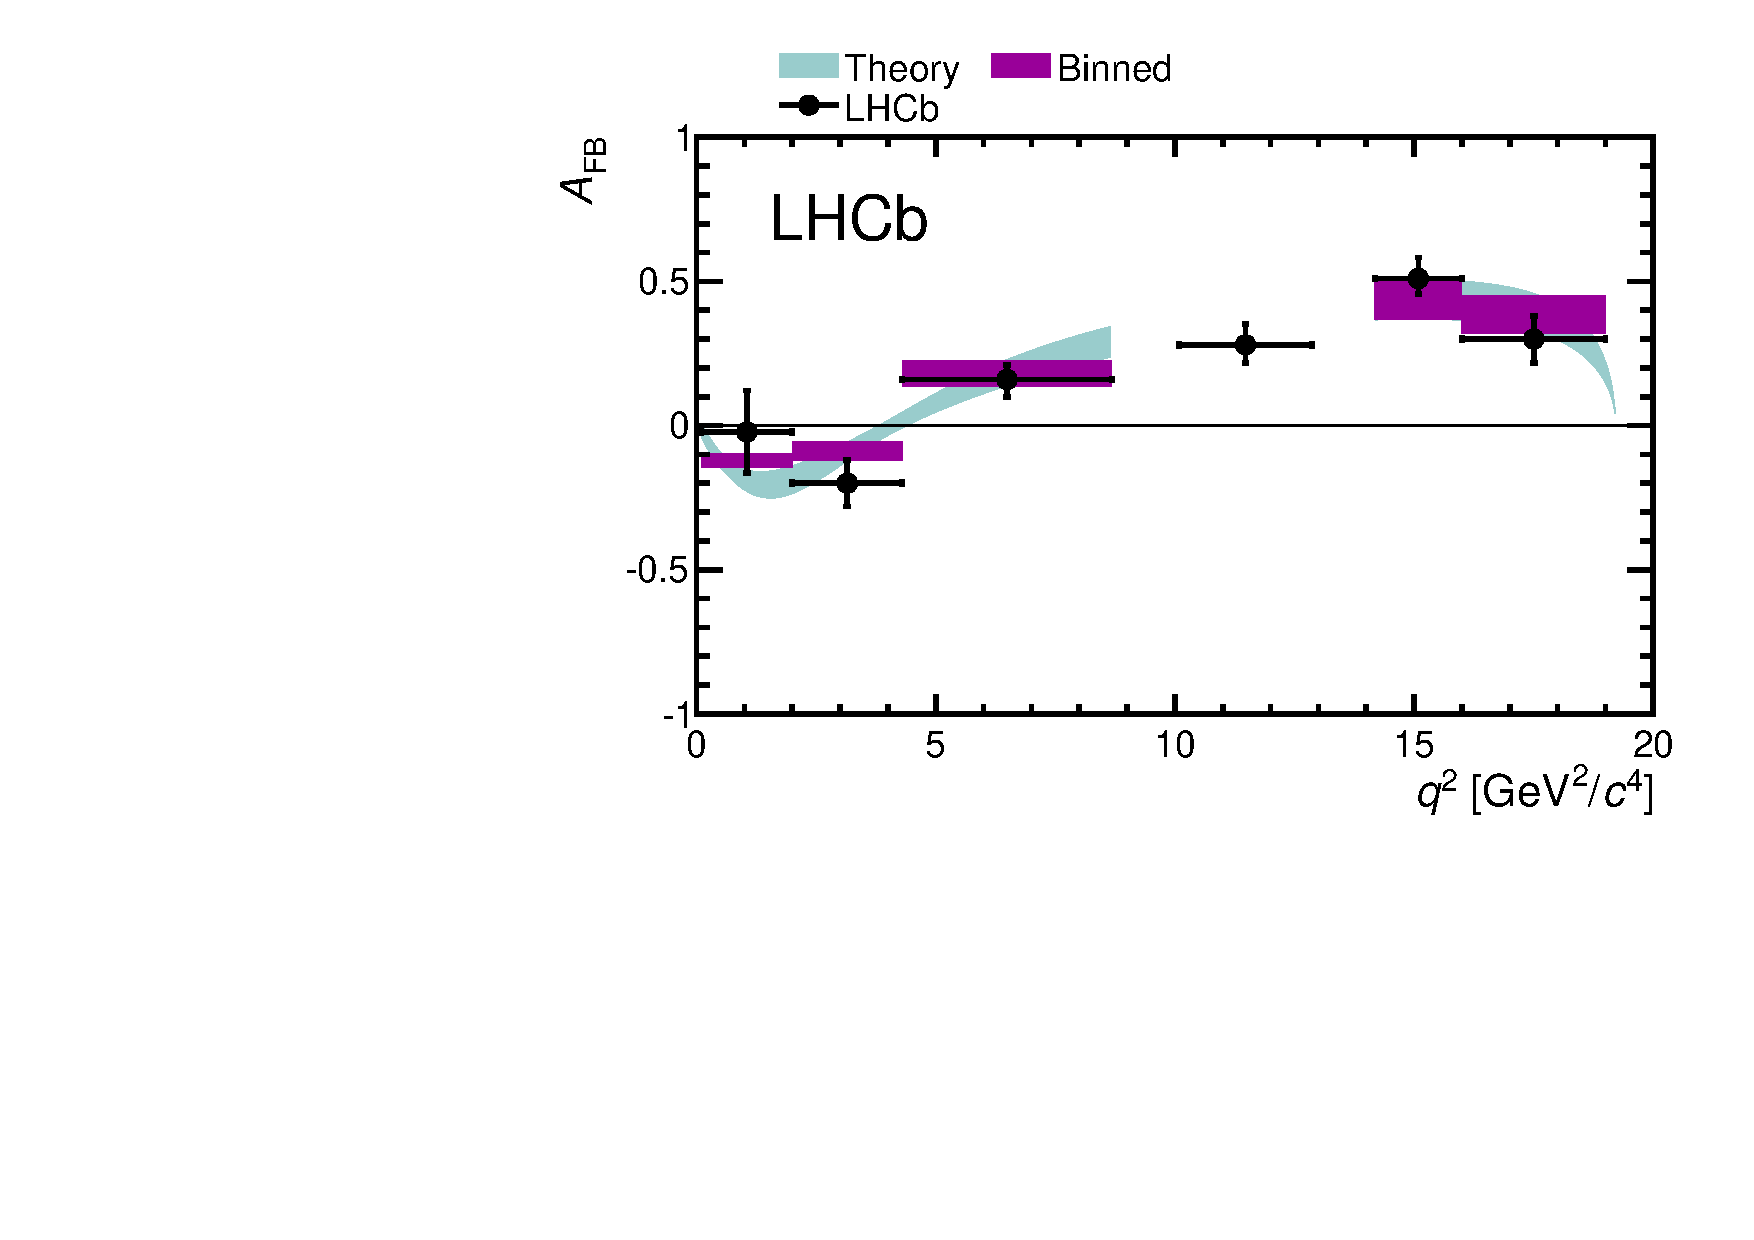
\includegraphics[scale=0.31]{chapter5/figs/paper2/cAFB.pdf}}
\subfigure[]{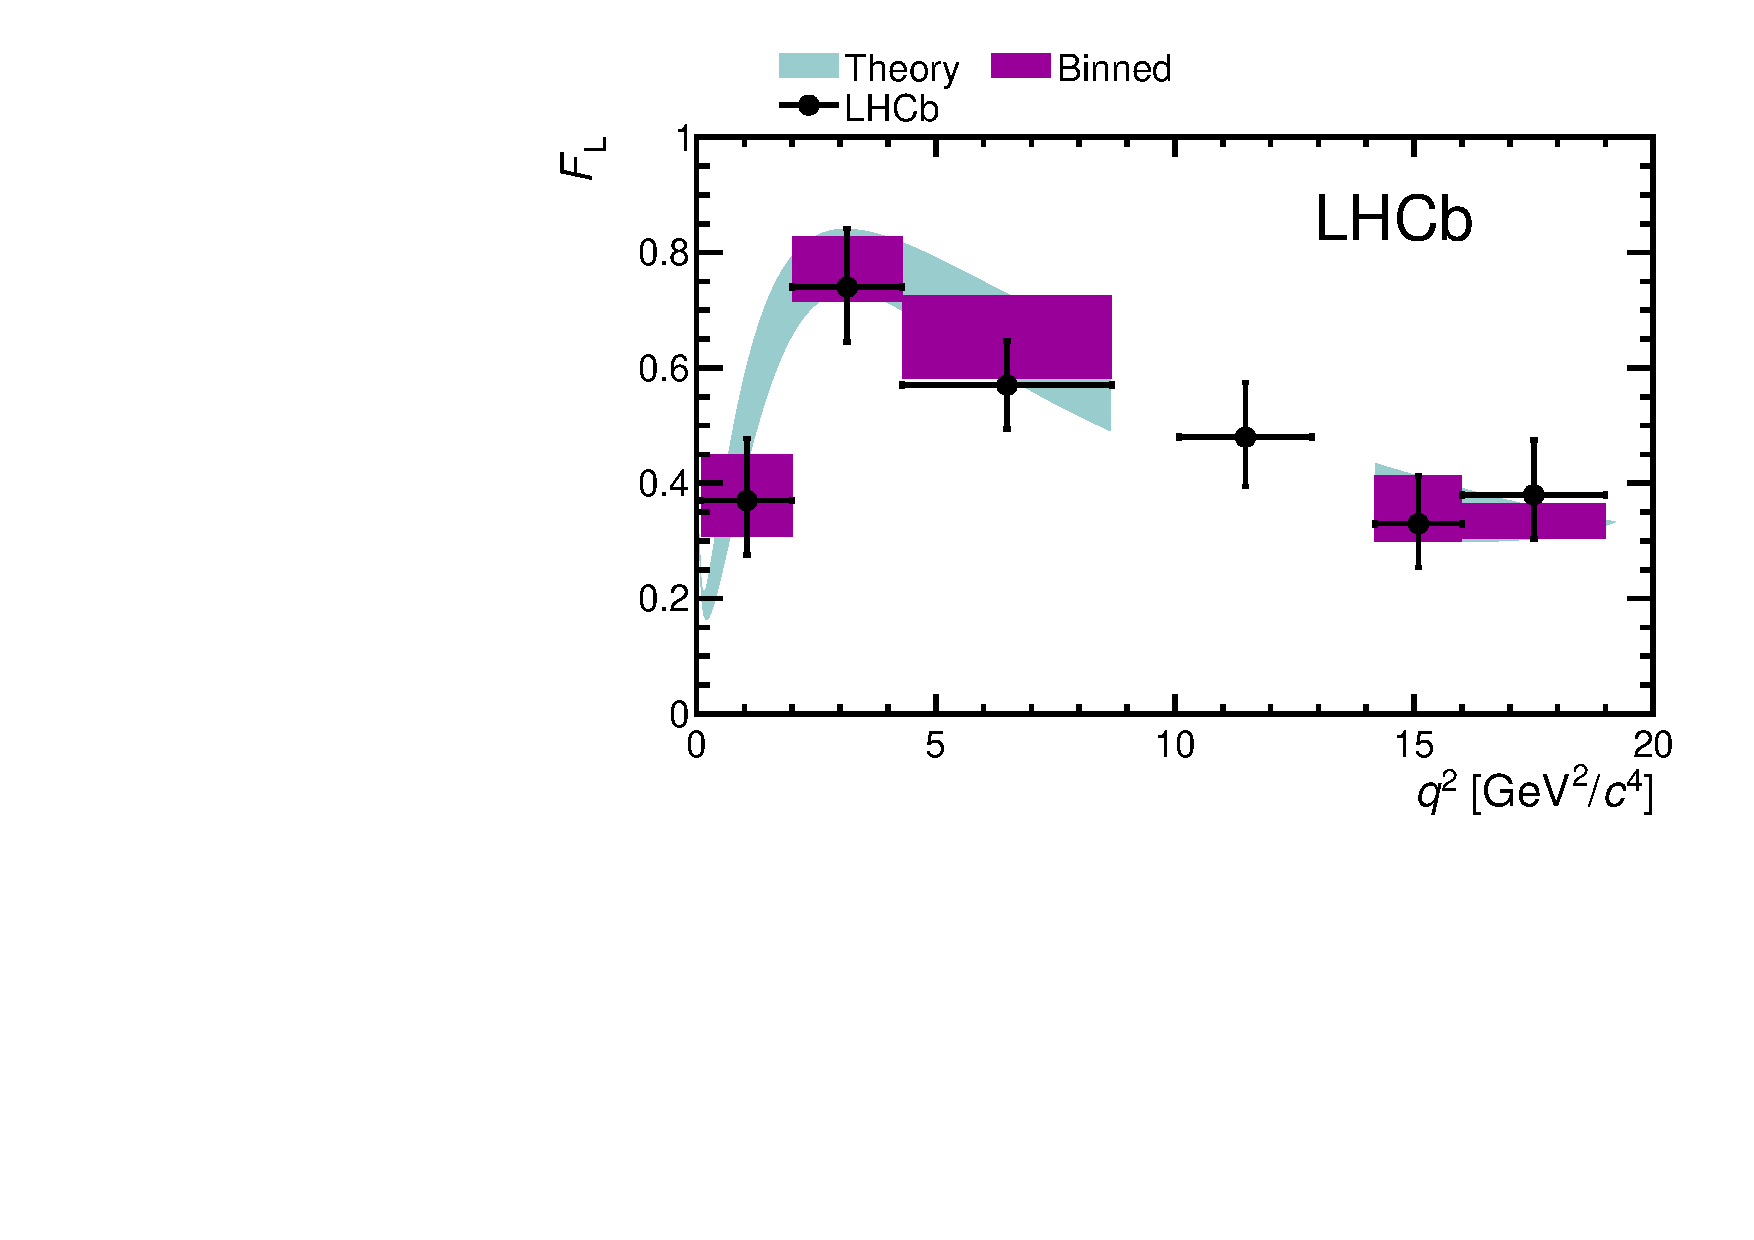
\includegraphics[scale=0.31]{chapter5/figs/paper2/cFL.pdf}}
\subfigure[]{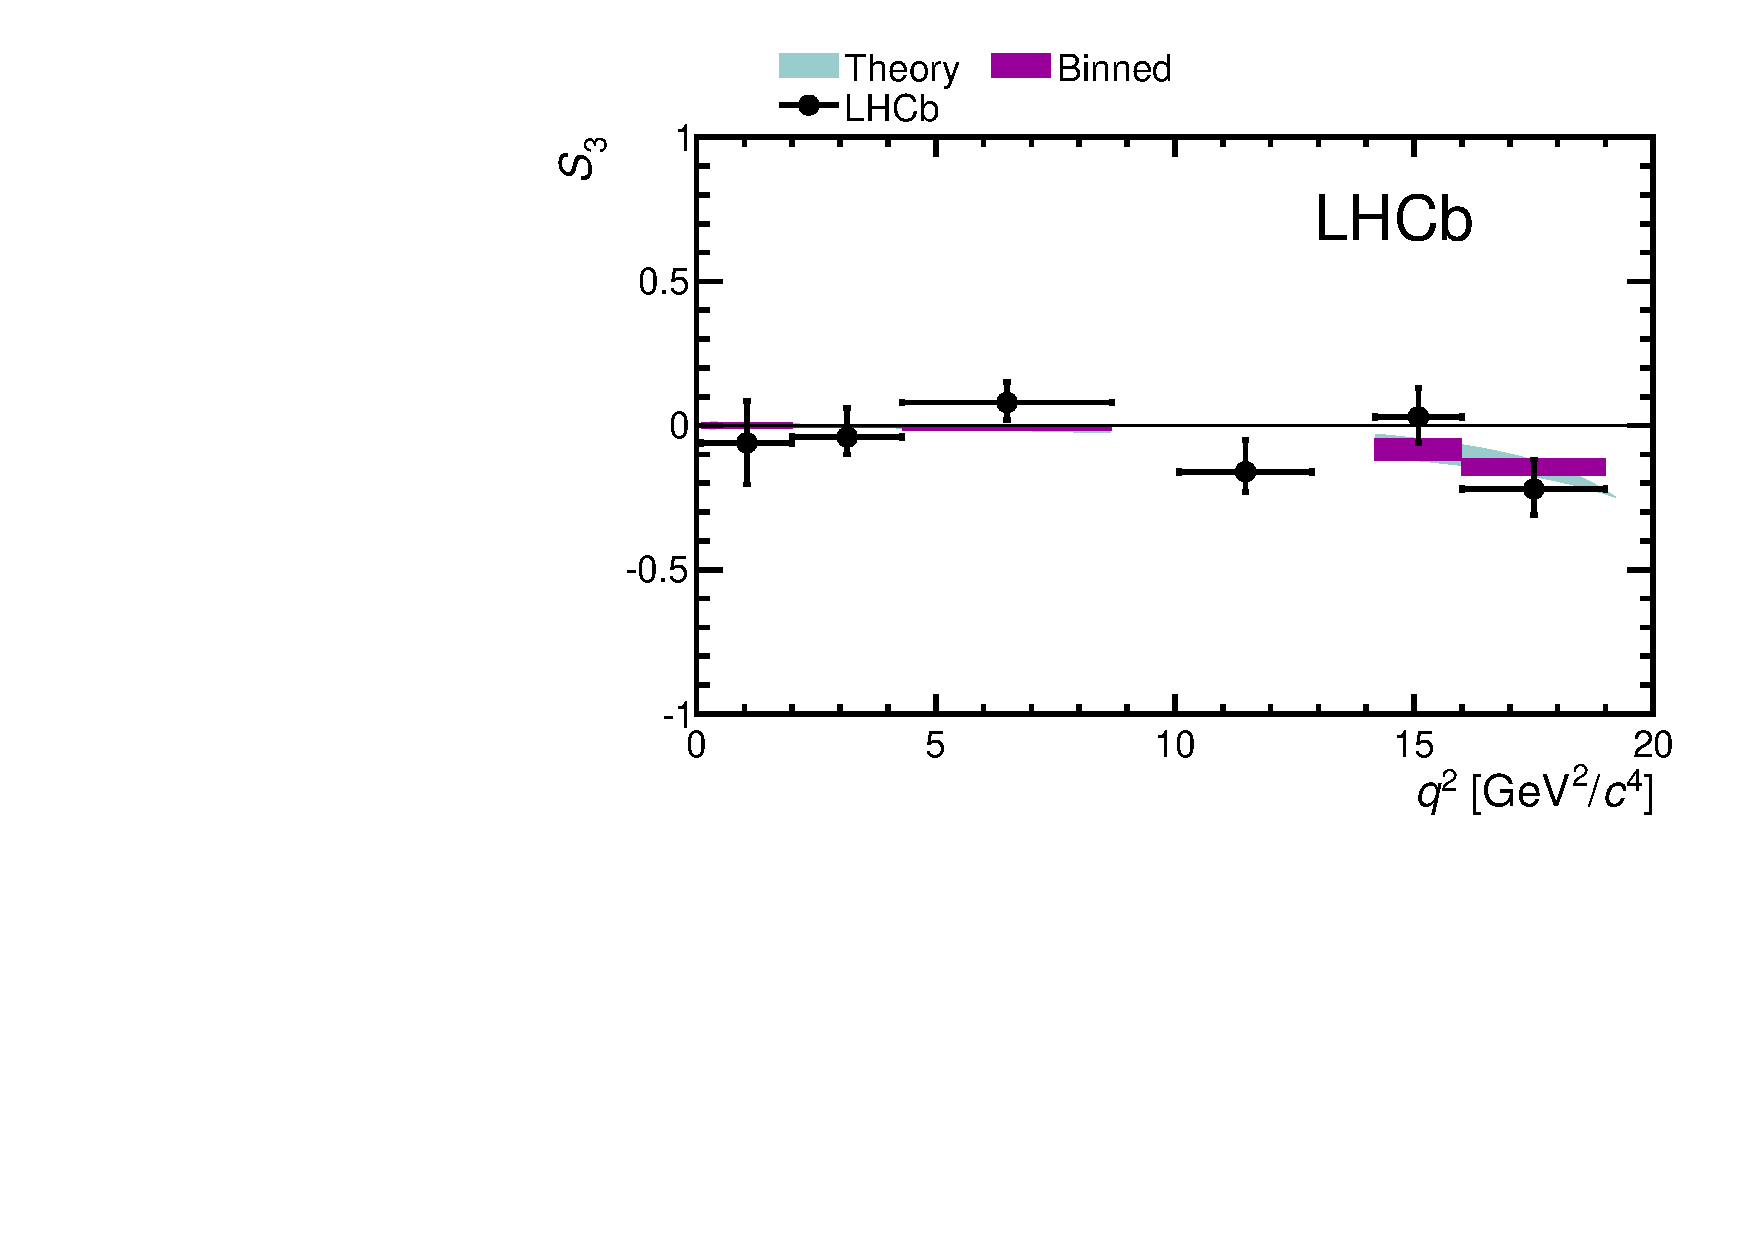
\includegraphics[scale=0.31]{chapter5/figs/paper2/cS3.pdf}}
\subfigure[]{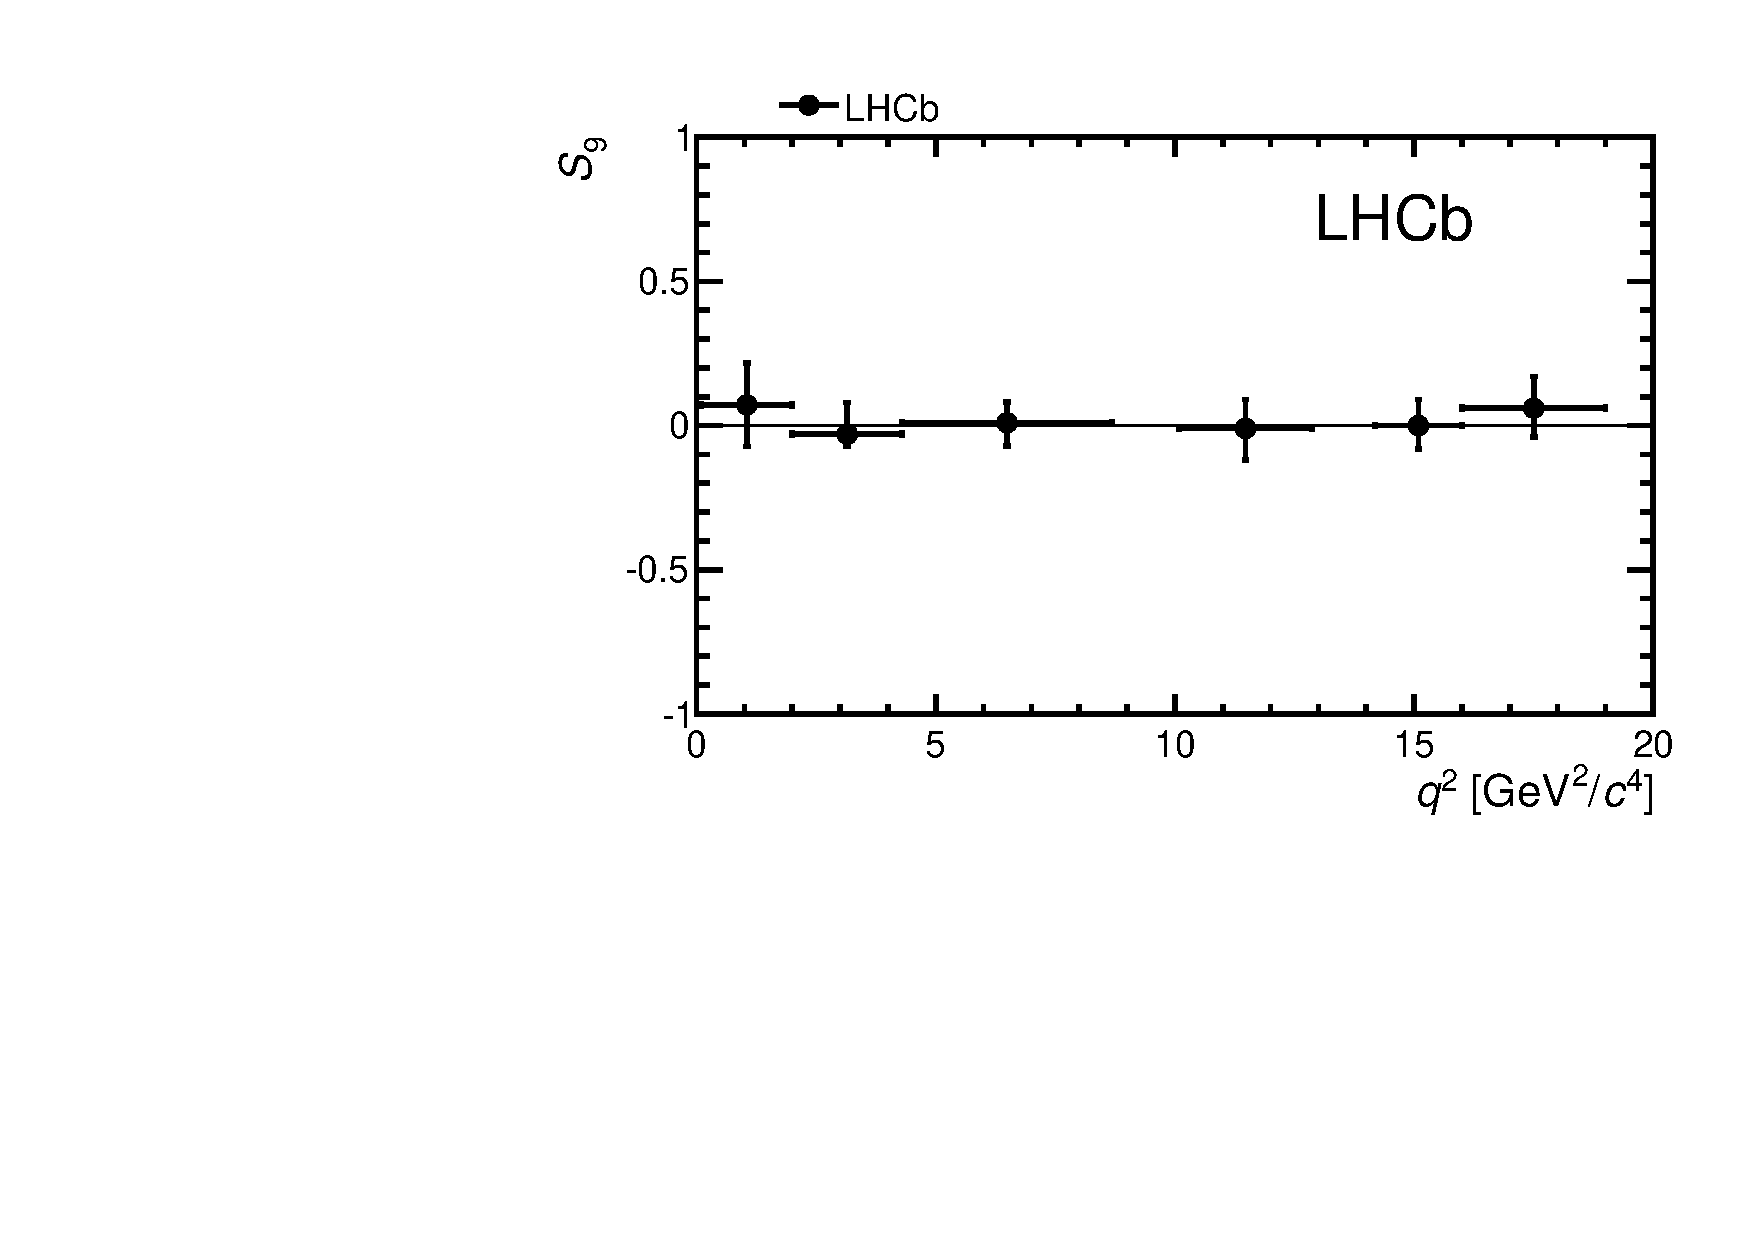
\includegraphics[scale=0.31]{chapter5/figs/paper2/cS9.pdf}}
\caption[ The final results from the angular analysis of \BdToKstmm at \lhcb using 1.0\invfb of data collected in 2011 at 7 \tev.   ]
{The final results from the angular analysis of \BdToKstmm at \lhcb using 1.0\invfb of data collected in 2011 at 7 \tev. 
Values for the original observables are extracted in the six different bins of \qsq.
The Standard Model prediction is from~\cite{Bobeth:2011gi}.
~\label{fig:kstmm:res2:norm}}
\end{figure}
\begin{figure}[tbp]
\centering
\subfigure[]{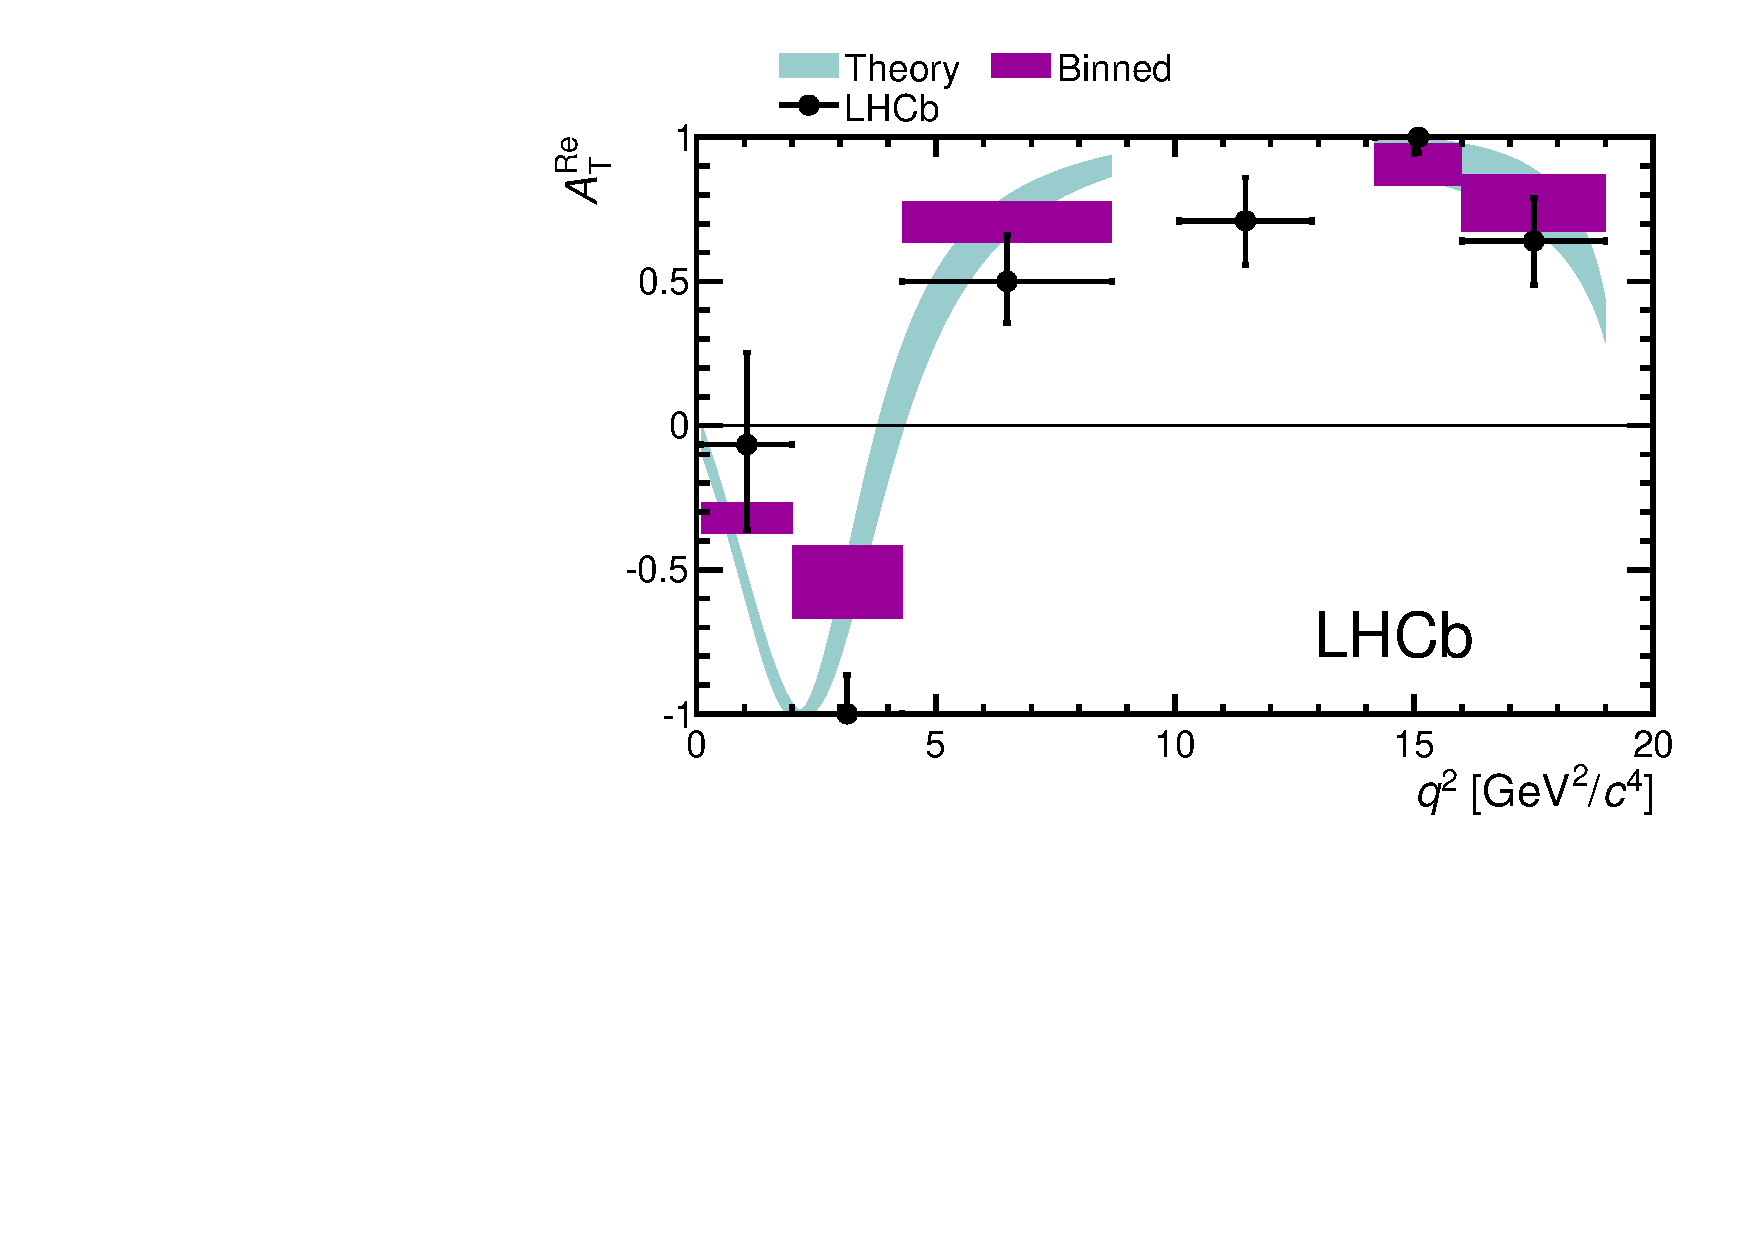
\includegraphics[scale=0.31]{chapter5/figs/paper2/cATRE.pdf}}
%\subfigure[]{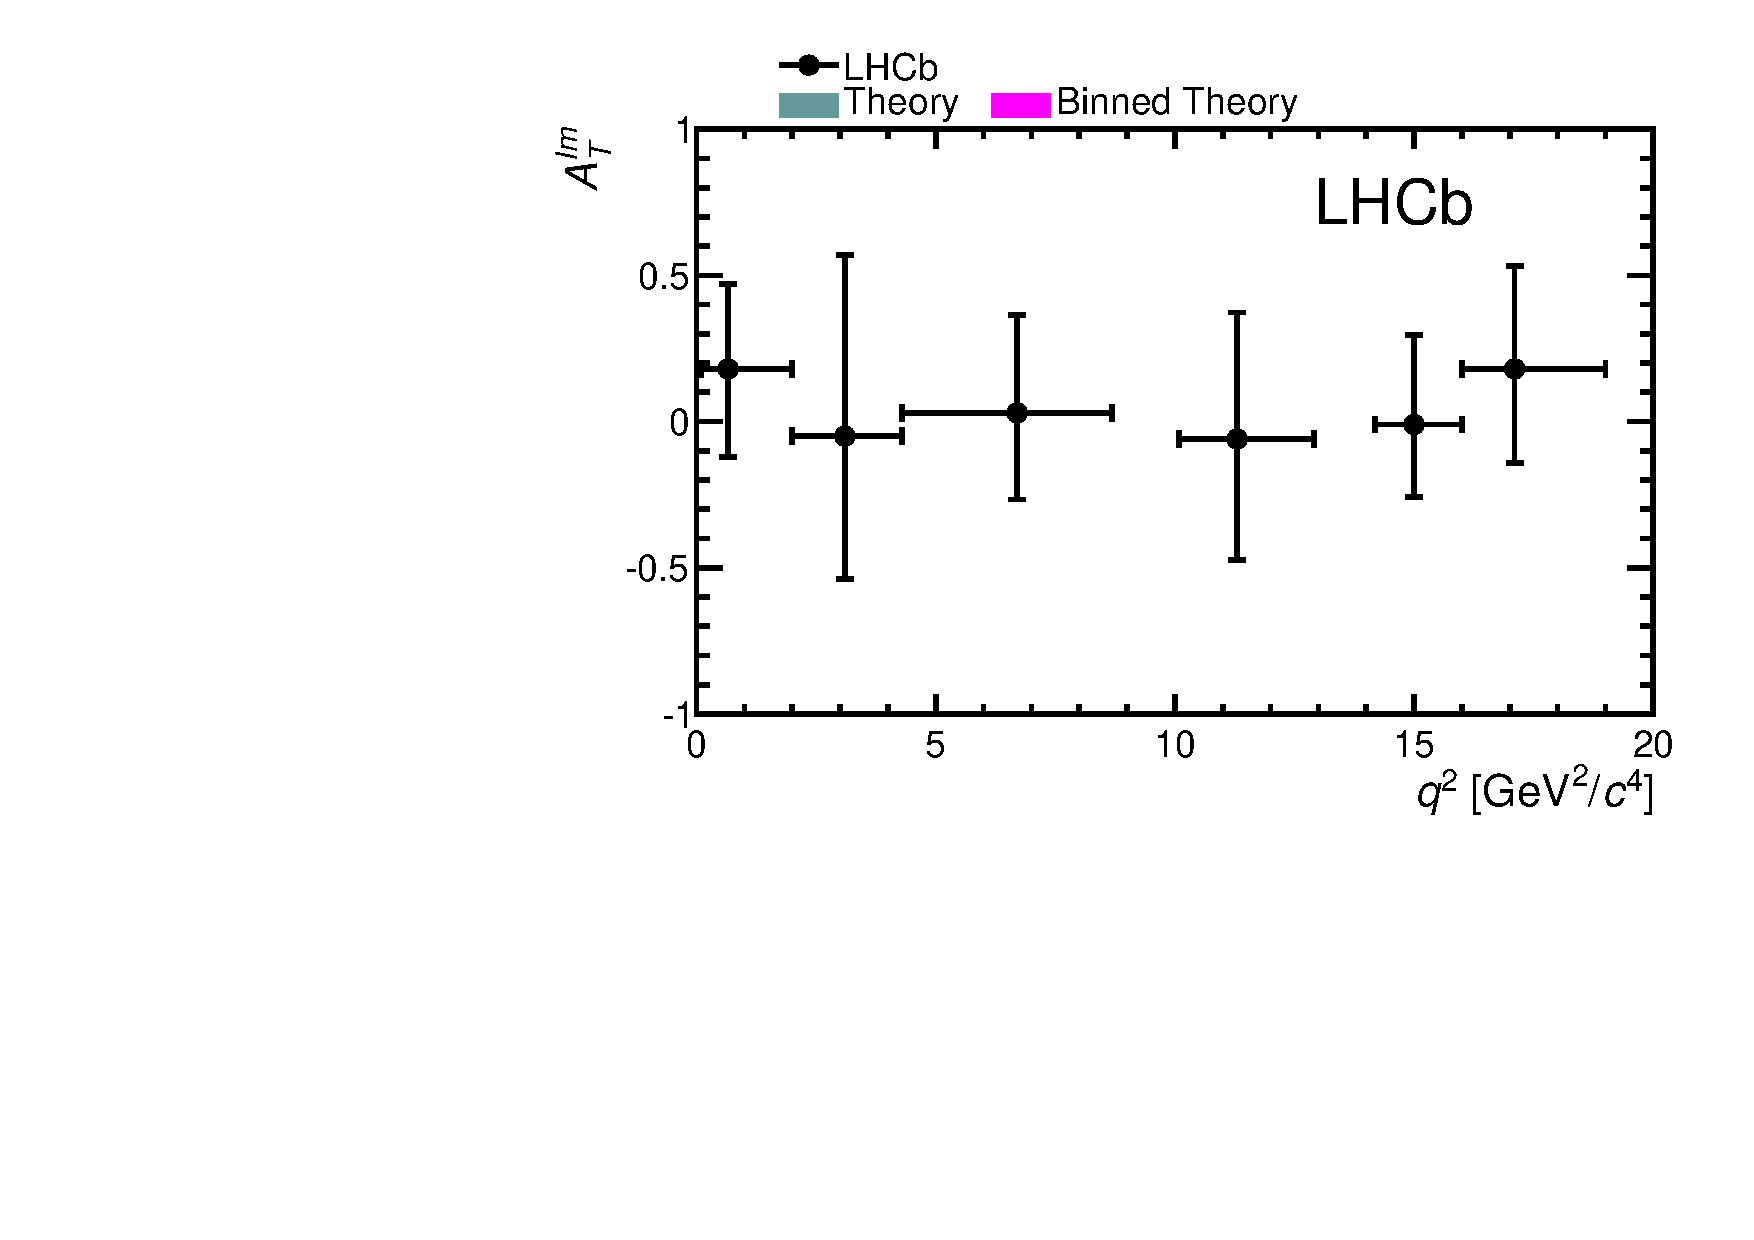
\includegraphics[scale=0.31]{chapter5/figs/results2/plot_ATI.pdf}}
\subfigure[]{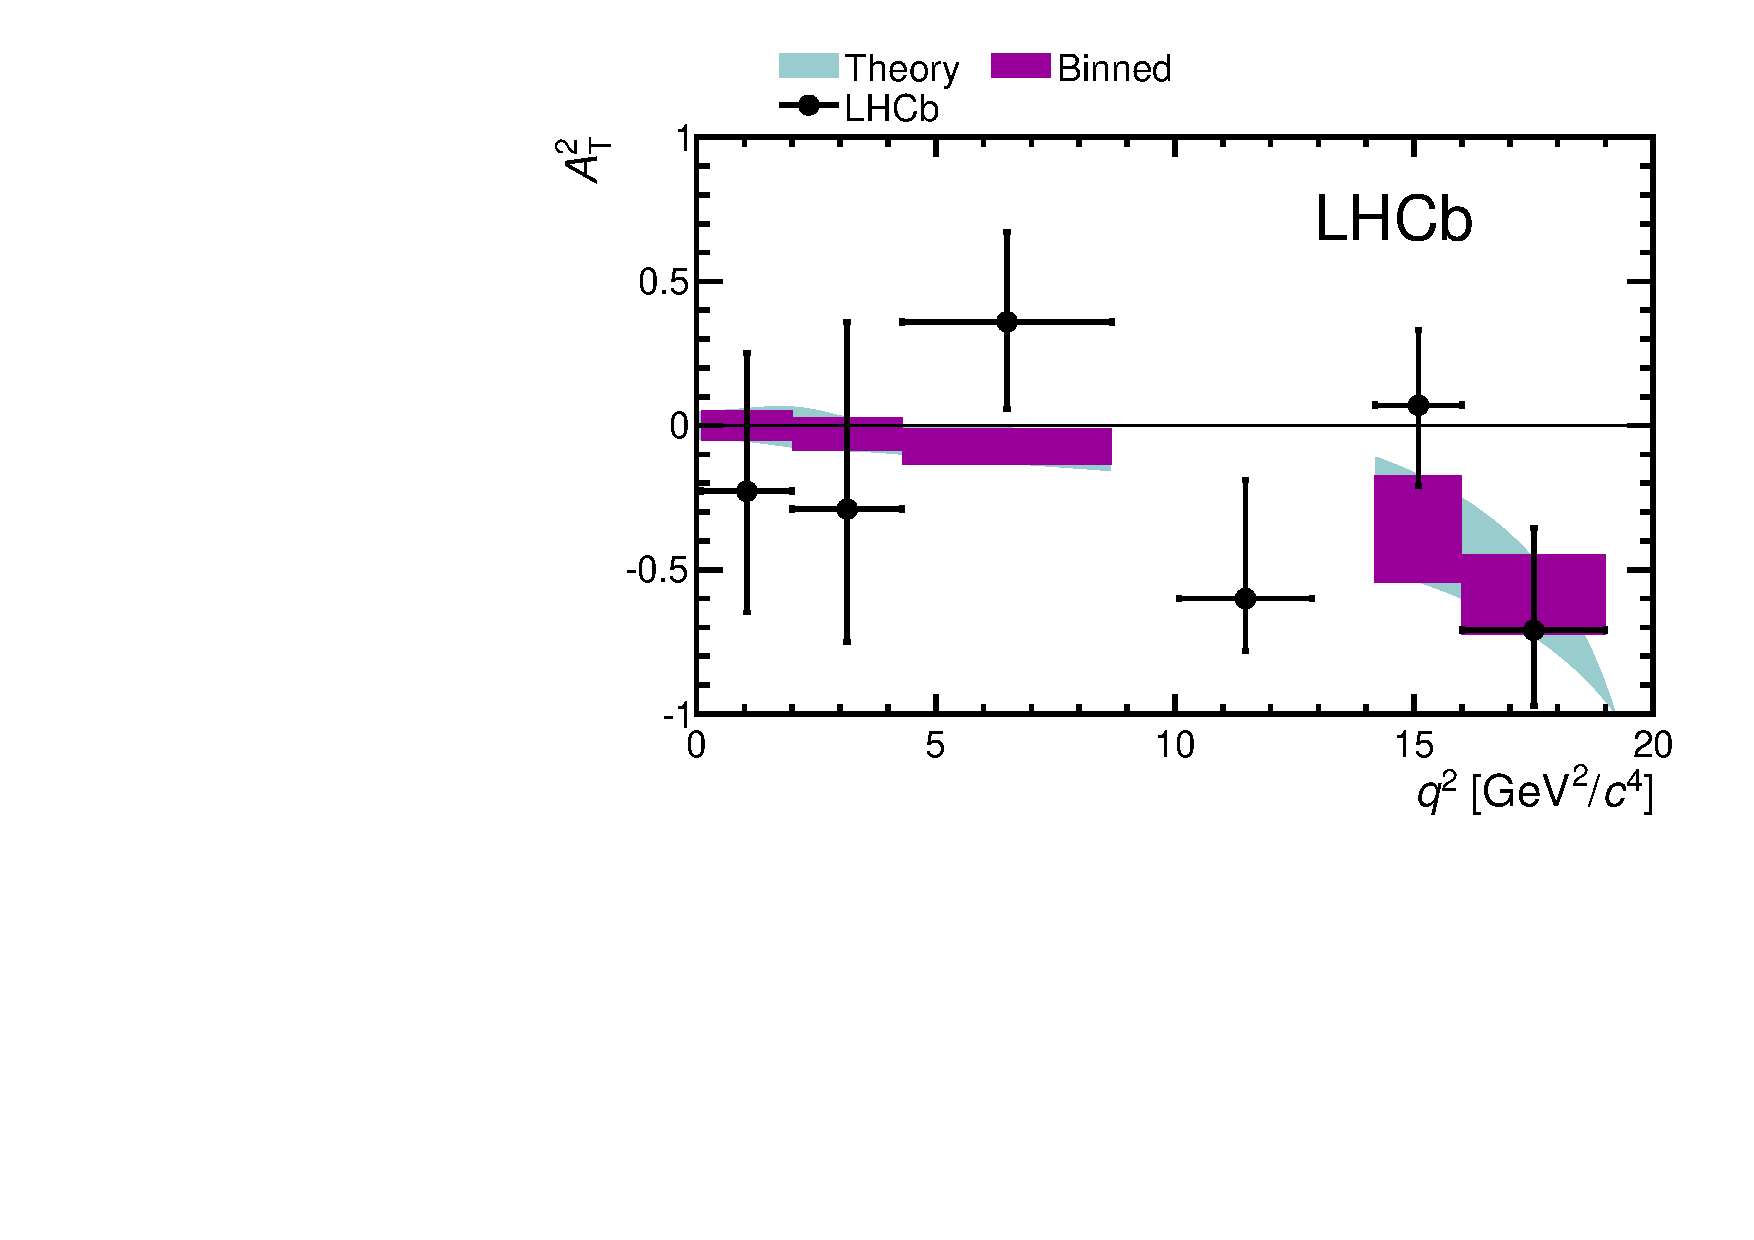
\includegraphics[scale=0.31]{chapter5/figs/paper2/cAT2.pdf}}
\subfigure[]{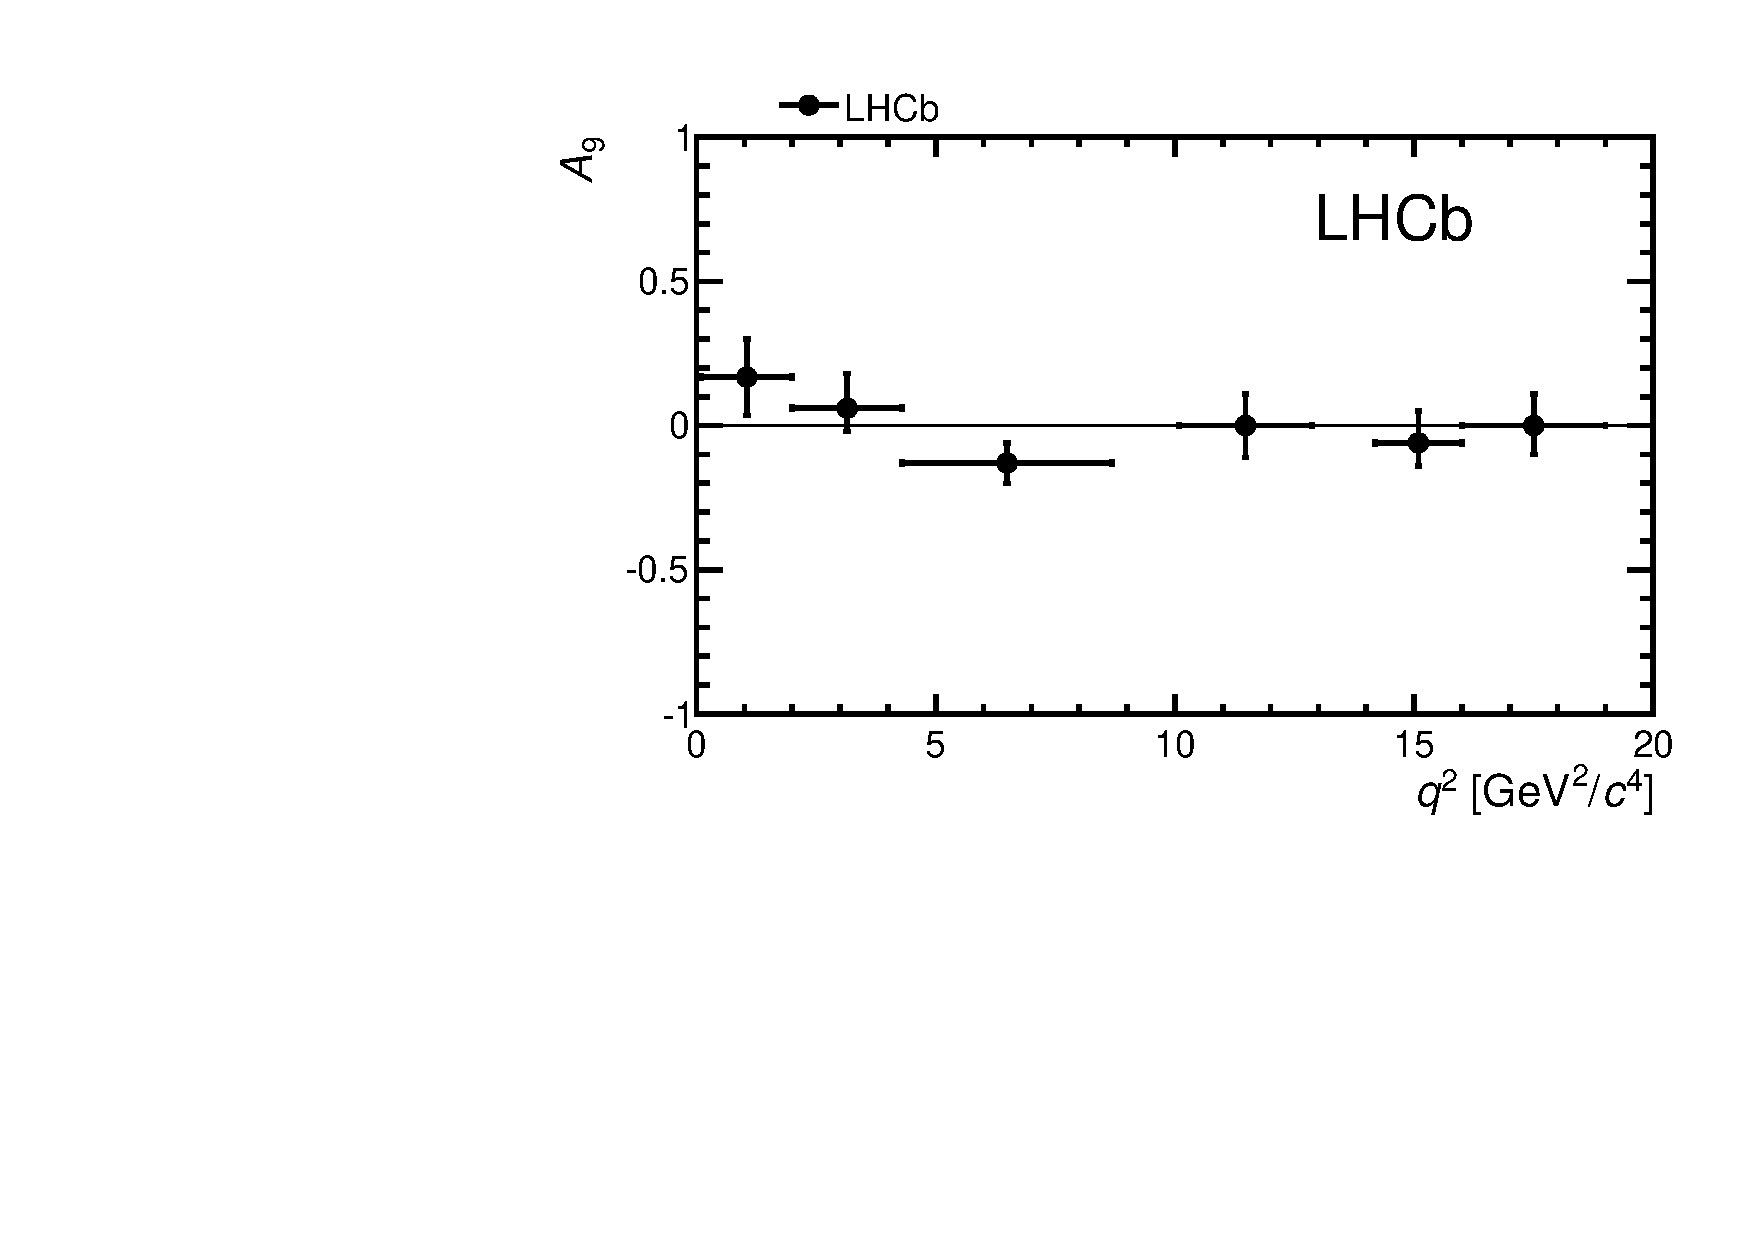
\includegraphics[scale=0.31]{chapter5/figs/paper2/cA9.pdf}}
%\subfigure[]{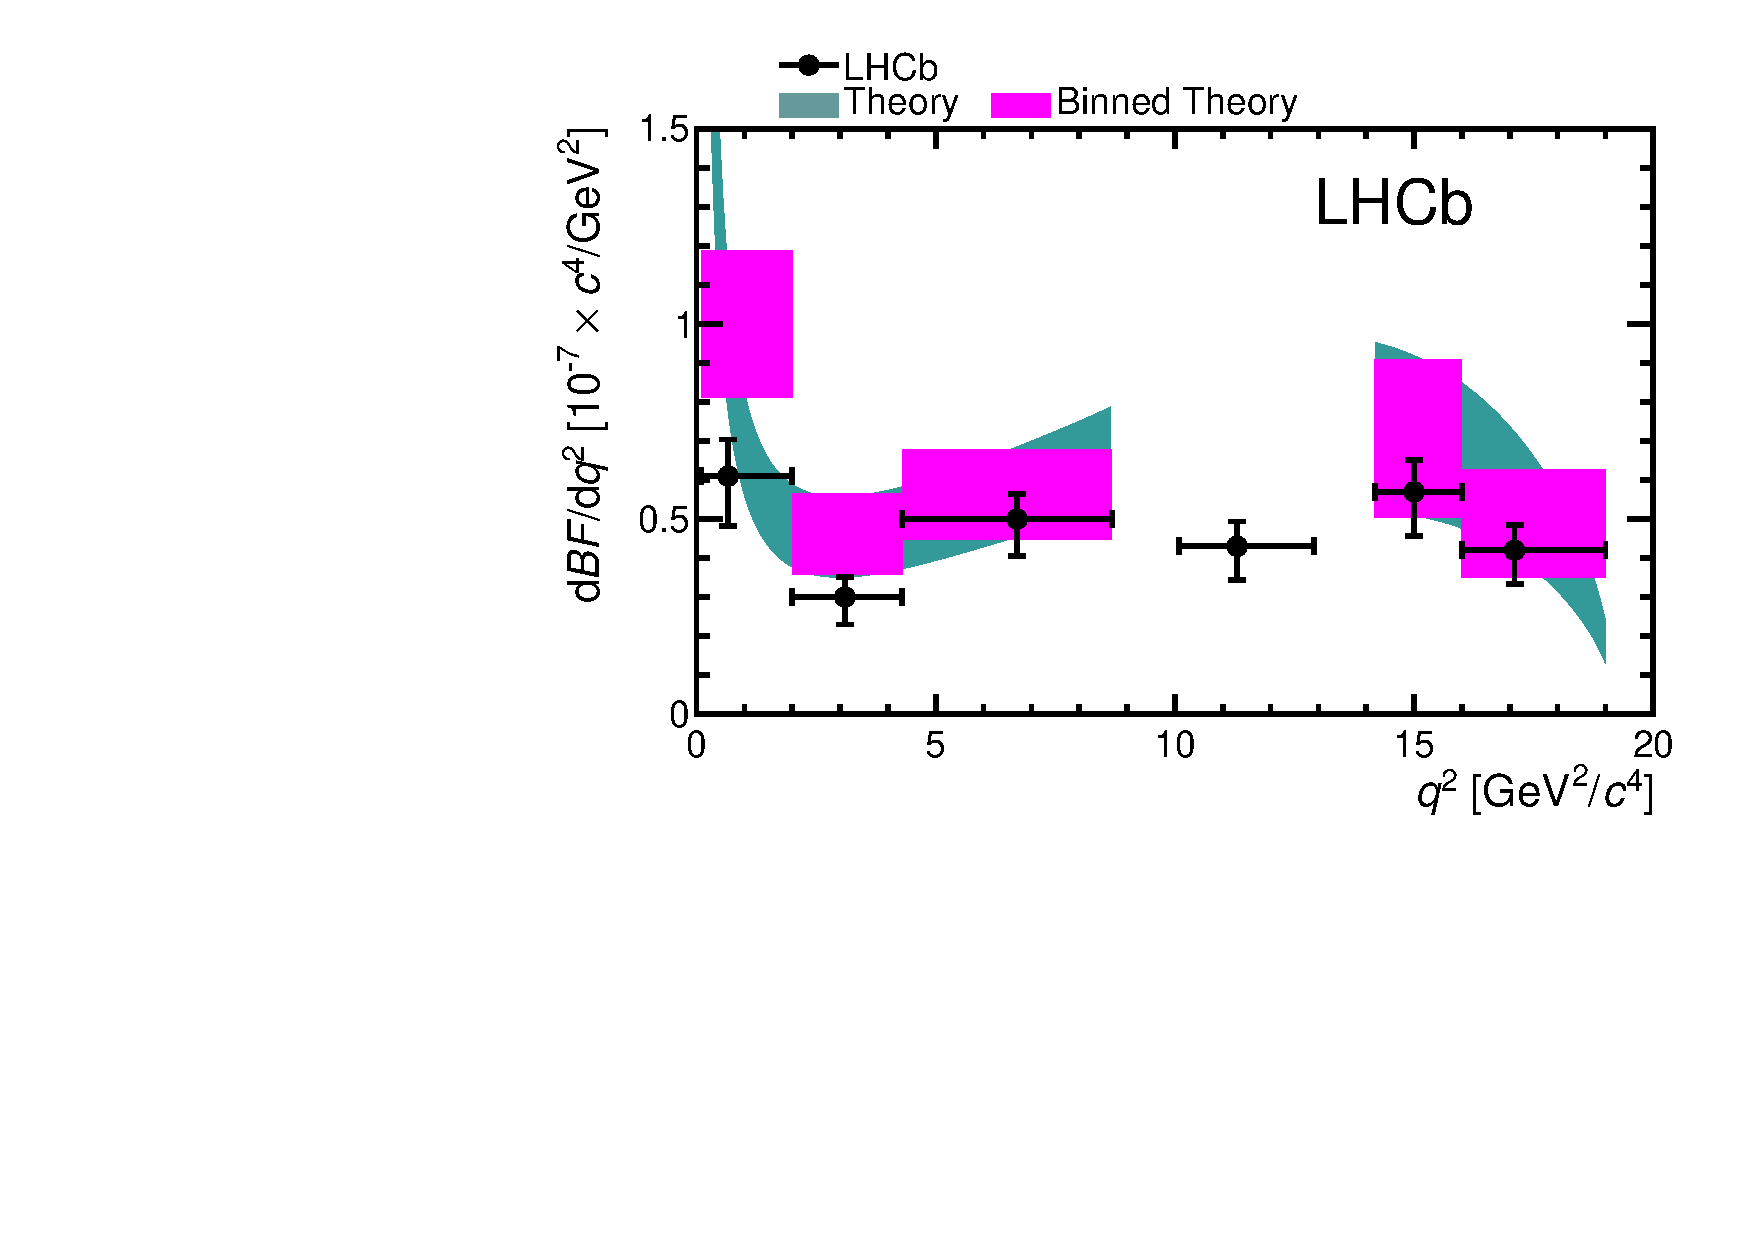
\includegraphics[scale=0.31]{chapter5/figs/results2/plot_Width.pdf}}
\caption[ The final results from the angular analysis of \BdToKstmm at \lhcb using 1.0\invfb of data collected in 2011 at 7 \tev.   ]
{The final results from the angular analysis of \BdToKstmm at \lhcb using 1.0\invfb of data collected in 2011 at 7 \tev. 
Values for the the reparameterised observables and the CP asymmetric observable \OA9 are extracted in the six different bins of \qsq.
The Standard Model prediction is from~\cite{Bobeth:2011gi}.
~\label{fig:kstmm:res2:reparam}}
\end{figure}
\begin{figure}[tbp]
\centering
\subfigure[]{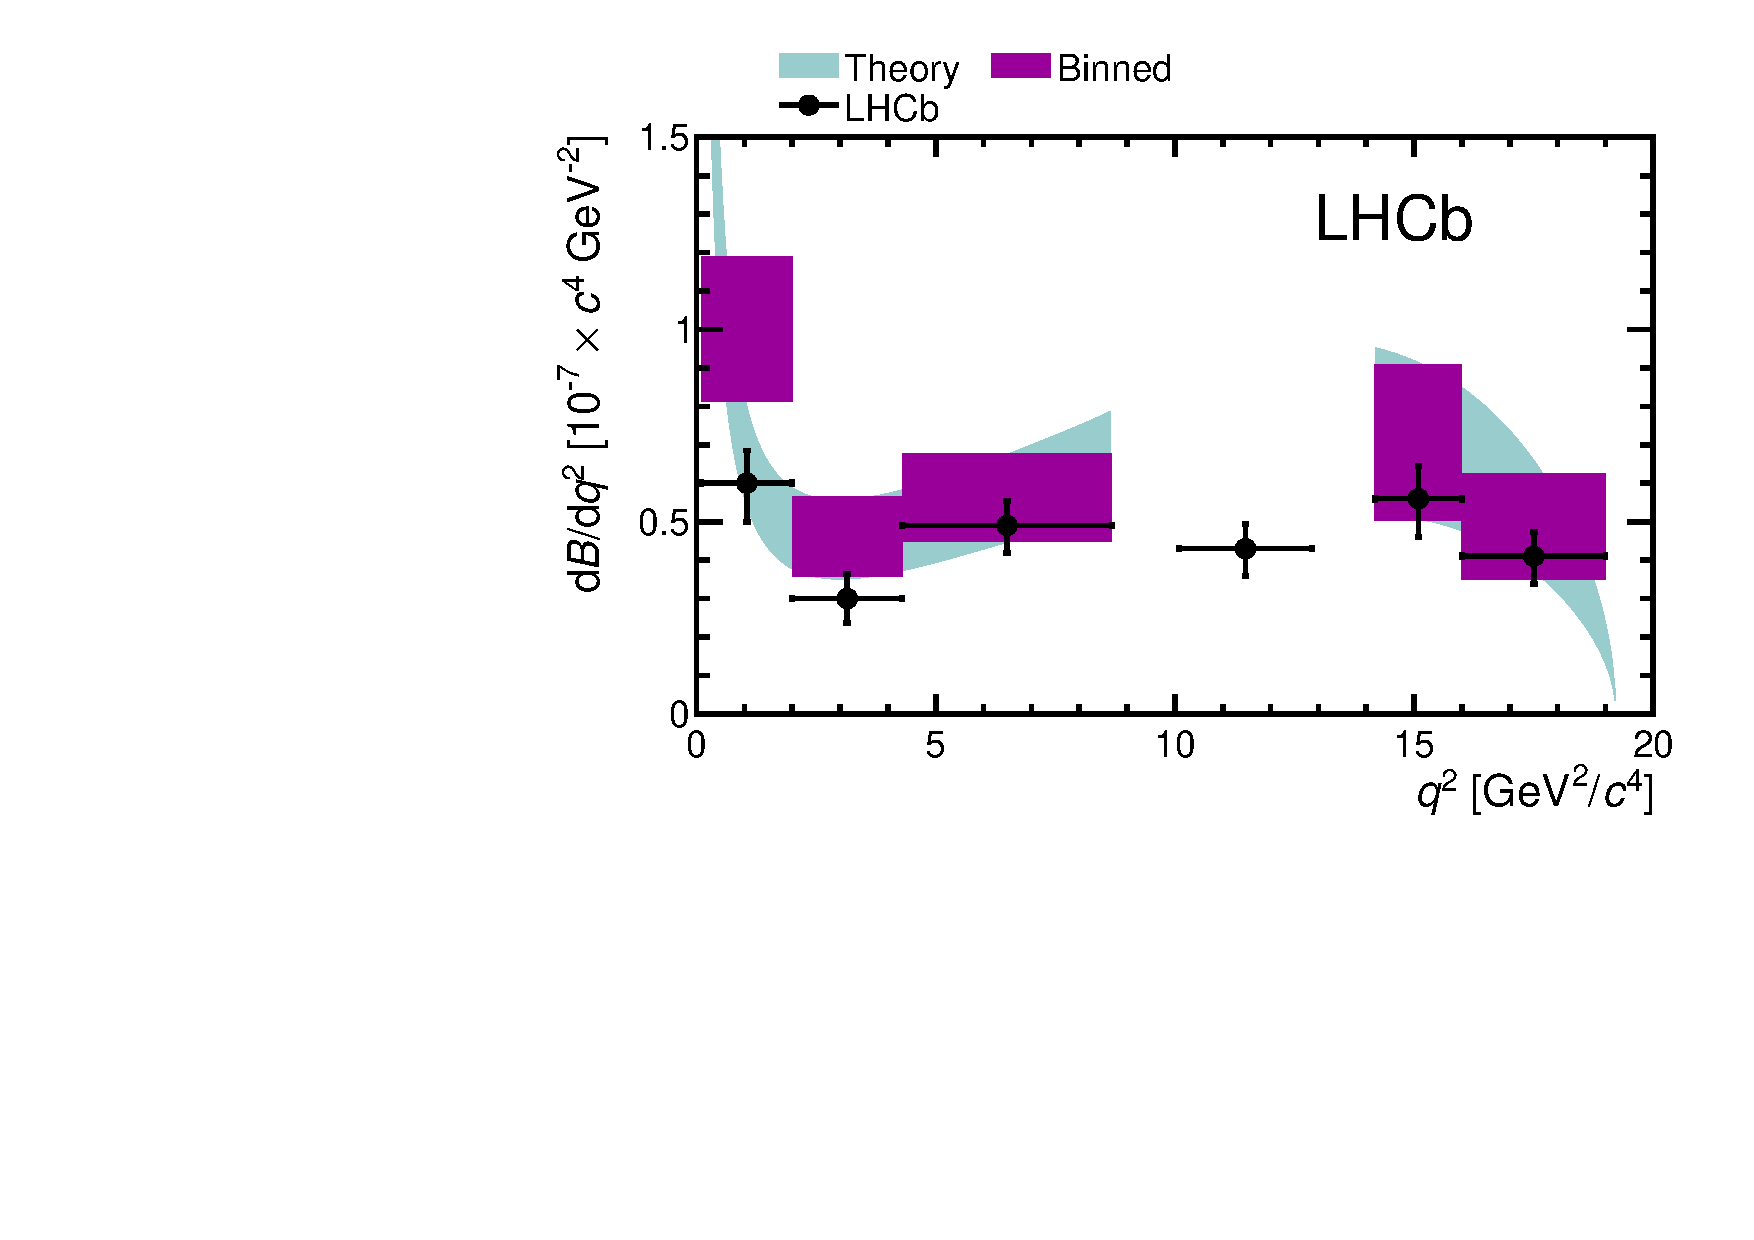
\includegraphics[scale=0.31]{chapter5/figs/paper2/cWidth.pdf}}
\caption[  The final results from the angular analysis of \BdToKstmm at \lhcb using 1.0\invfb of data collected in 2011 at 7 \tev.  ]
{The final results from the angular analysis of \BdToKstmm at \lhcb using 1.0\invfb of data collected in 2011 at 7 \tev. 
The differential branching fraction is extracted in the six different bins of \qsq.
The Standard Model prediction is from~\cite{Bobeth:2011gi}.
~\label{fig:kstmm:res2:a9dbr}}
\end{figure}











